% Appendix D: details of Claim 1 (later mentions decide the route). Input by sections/appendix.tex.
\section{Later mentions decide the route: details}\label{app:claim1}

\subsection{The discovery sample}\label{app:discovery}\label{sec:read}\label{sec:mentions}\label{sec:general}\label{app:additional}

The discovery sample is the \nModels{} models and the story cores of entries A--I: Qwen2.5-Instruct at 1.5B, 3B, 7B, 14B, 32B and 72B, Qwen3-8B, Mistral-7B, Mistral-Small-24B and OLMo-2-7B (three developers), with 150 stories per format and model unless stated. Its results are reported as they were scored in the earlier entries, with their labels: a preregistered result names its prediction (B1 is prediction~1 of preregistration~B; \cref{app:prereg-ai}), and the others are marked exploratory or post hoc. These results use the lower-case score; the final round re-scored the five discovery-sample verdicts that depend on the scoring and found every one unchanged under the forms the models emit (\cref{app:measure}). Unless stated otherwise, intervals are 95\% percentile intervals from 10{,}000 bootstrap resamples of stories (cores), with ratios recomputed within each resample. Each estimate is printed with its interval below it, except in \cref{tab:onset,tab:decomposition}, where the intervals of the individual effects are in the result summaries released with the code.

\paragraph{Natural formats.}
Over all \nModels{} models (\cref{tab:natural}), the formats fall into three regimes.

\emph{Candidates listed after the writing token.} Under \fmtOpt{} and \fmtLetter{}, $\mathrm{ID}_K$ is large and positive in every model, from \idKOptQwenOnefive{} nats at Qwen2.5-1.5B to \idKOptQwenFourteen{} at Qwen2.5-14B under \fmtOpt{} (A1 at 1.5B on new cores of seed~1 and B1 in five held-out models from 3B to 8B, both met; exploratory at 14B and 24--72B).

\emph{No later mention.} Under \fmtNone{}, $\mathrm{ID}_K$ is at most \noneMax{} nats, less than a tenth of its \fmtOpt{} value in every model (paired difference positive in 5/5 held-out models; B2, met), and the identity is mainly copied: $\mathrm{ID}_V$ exceeds $\mathrm{ID}_K$ more than tenfold (exploratory; \cref{tab:decomposition}). \fmtBefore{} names the same candidates before the writing token, which the causal mask keeps them from attending to; its $\mathrm{ID}_K$ is never reliably positive, and negative in nine of ten models (C4's 0.5-nat bound met; sign unexplained).

\emph{A neutral sentence after the story.} \fmtPost{} carries no positive key identity at Qwen2.5-1.5B and 3B, but an intermediate amount in every model from 7B up (\idKPostOlmoSeven{}--\idKPostQwenFourteen{} nats), which we did not predict. The scale-free identity key share $s_{\mathrm{ID}}$ above 1.5B is \idShareOptMinNoOnefive{}--\idShareOptMax{} under \fmtOpt{} and at most \idSharePostMax{} under \fmtPost{} and \idShareNoneMax{} under \fmtNone{} (exploratory; \cref{tab:idshare}).

\begin{table}[!ht]
  \centering
  \caption{\textbf{Position decides the key read} (discovery sample: the stories of stages 1 and 3b). The same list or neutral sentence, after or before the story, with ``Answer with one word''; \fmtNone{} for reference. $\mathrm{ID}_K$ (nats, 95\% CIs), $n = 150$, keys clamped from layer~0. Preregistration~E (E1).}
  \label{tab:twobytwo}
  {\footnotesize\setlength{\tabcolsep}{4pt}\begin{tabular}{@{}lcccc@{}}
\toprule
Format & Qwen-7B & Qwen-14B & Mistral-7B & OLMo-2-7B \\
\midrule
\fmtListA & \begin{tabular}[t]{@{}c@{}}+20.6\\[-1pt]{\scriptsize[20.2, 21.0]}\end{tabular} & \begin{tabular}[t]{@{}c@{}}+35.8\\[-1pt]{\scriptsize[34.9, 36.7]}\end{tabular} & \begin{tabular}[t]{@{}c@{}}+15.6\\[-1pt]{\scriptsize[15.1, 16.0]}\end{tabular} & \begin{tabular}[t]{@{}c@{}}+8.7\\[-1pt]{\scriptsize[8.4, 8.9]}\end{tabular} \\
\fmtPost & \begin{tabular}[t]{@{}c@{}}+5.5\\[-1pt]{\scriptsize[5.2, 5.8]}\end{tabular} & \begin{tabular}[t]{@{}c@{}}+12.1\\[-1pt]{\scriptsize[11.5, 12.7]}\end{tabular} & \begin{tabular}[t]{@{}c@{}}+7.9\\[-1pt]{\scriptsize[7.3, 8.4]}\end{tabular} & \begin{tabular}[t]{@{}c@{}}+2.0\\[-1pt]{\scriptsize[1.8, 2.2]}\end{tabular} \\
\fmtBefore & \begin{tabular}[t]{@{}c@{}}$-$0.1\\[-1pt]{\scriptsize[$-$0.2, $-$0.1]}\end{tabular} & \begin{tabular}[t]{@{}c@{}}$-$0.1\\[-1pt]{\scriptsize[$-$0.2, 0.0]}\end{tabular} & \begin{tabular}[t]{@{}c@{}}0.0\\[-1pt]{\scriptsize[$-$0.1, 0.1]}\end{tabular} & \begin{tabular}[t]{@{}c@{}}$-$0.3\\[-1pt]{\scriptsize[$-$0.4, $-$0.2]}\end{tabular} \\
\fmtSentB & \begin{tabular}[t]{@{}c@{}}0.0\\[-1pt]{\scriptsize[$-$0.1, 0.1]}\end{tabular} & \begin{tabular}[t]{@{}c@{}}$-$0.1\\[-1pt]{\scriptsize[$-$0.2, 0.0]}\end{tabular} & \begin{tabular}[t]{@{}c@{}}0.0\\[-1pt]{\scriptsize[$-$0.1, 0.1]}\end{tabular} & \begin{tabular}[t]{@{}c@{}}$-$0.2\\[-1pt]{\scriptsize[$-$0.3, $-$0.2]}\end{tabular} \\
\midrule
\fmtNone & \begin{tabular}[t]{@{}c@{}}+1.0\\[-1pt]{\scriptsize[0.9, 1.2]}\end{tabular} & \begin{tabular}[t]{@{}c@{}}+1.1\\[-1pt]{\scriptsize[0.9, 1.2]}\end{tabular} & \begin{tabular}[t]{@{}c@{}}+0.6\\[-1pt]{\scriptsize[0.5, 0.6]}\end{tabular} & \begin{tabular}[t]{@{}c@{}}+0.4\\[-1pt]{\scriptsize[0.3, 0.5]}\end{tabular} \\
\bottomrule
\end{tabular}
}
\end{table}

\paragraph{An instruction-matched $2{\times}2$.}
Preregistration~E crosses \{list, sentence\} with \{before, after\} under one instruction (\cref{tab:twobytwo}); all parts of E1 were met. $\mathrm{ID}_K$ is \twoAfterMin{}--\twoAfterMax{} nats under \fmtListA{} and \twoPostMin{}--\twoPostMax{} under \fmtPost{}, every CI before the story contains zero or lies below it, and both paired differences exclude zero in 4/4 models. Position, not the instruction or the list format, decides whether the key channel opens.

\paragraph{Across tasks, families and scale.}
On the paint and schedule tasks, in five 7--14B models, the paired \fmtOpt{}$-$\fmtNone{} difference in $\mathrm{ID}_K$ is positive in 5/5 models per task (D1, met), and \fmtBefore{} stays within the preregistered 0.5-nat bound in 10/10 cells (D2, met; \cref{tab:tasks}). On IOI \citep{wang2022ioi}, plain sentences carry almost no key identity (G18, met), but the preregistered test that a later list opens a key read was not met (G19; Mistral-7B failed the competence gate; \cref{app:g-ioi}). Within Qwen2.5, the \fmtOpt{} key share $s_K$ rises from \shareQwenOnefive{} at 1.5B to \shareQwenFourteen{} at 14B and falls to \shareQwenSeventytwo{} at 72B (B3, exploratory; \cref{fig:scale}). The fall is not an artefact of the software or GPU setup (E3, met), but its cause is unknown. Other families give \shareOlmoSeven{}--\shareMistralSeven{} (deeper clamp onsets: \cref{tab:onset}).

\paragraph{Natural factorial in all models.} \Cref{tab:natural} gives the \fmtOpt{} key share and $\mathrm{ID}_K$ in every format for all \nModels{} models, and \cref{fig:formats} shows $\mathrm{ID}_K$ relative to \fmtOpt{}. \fmtBefore{} is negative in every model except Mistral-7B, where it is indistinguishable from zero; at Qwen2.5-72B it reaches $\idKBeforeQwenSeventytwo$ nats.

\begin{table}[!ht]
\centering
\caption{\textbf{Natural factorial, all models.} Key share $s_K$ under \fmtOpt{} and value identity carried by keys, $\mathrm{ID}_K$ (nats), in each format, with keys and values clamped from layer~0. $n = 150$ stories per format and model; 95\% bootstrap CIs over stories (ratio recomputed in each resample for $s_K$). Models ordered by size. Rows up to 14B are from GPU stage 1, whose predictions B1--B2 cover \fmtOpt{}, \fmtLetter{} and \fmtNone{} in Qwen2.5-3B/7B, Qwen3-8B, Mistral-7B and OLMo-2-7B; rows from 24B are from stage 2, whose prediction C4 covers $s_K$ and \fmtBefore{}. The other cells, including the 1.5B and 14B rows, are exploratory; preregistration A tested 1.5B in a separate run (\cref{tab:prereg-ab}).}
\label{tab:natural}
\resizebox{\textwidth}{!}{\begin{tabular}{lcccccc}
\toprule
Model & key share (P1) & \multicolumn{5}{c}{identity carried by keys (nats)} \\
\cmidrule(lr){3-7}
 & & lettered & options after & re-mention & none & options before \\
\midrule
Qwen2.5-1.5B & 0.37 [0.36, 0.39] & +3.6 & +2.8 & -0.5 & +0.2 & -0.2 \\
Qwen2.5-3B & 0.69 [0.68, 0.71] & +11.4 & +10.3 & -0.0 & +0.1 & -0.5 \\
Mistral-7B & 0.92 [0.90, 0.93] & +15.2 & +14.9 & +7.9 & +0.6 & +0.0 \\
OLMo-2-7B & 0.73 [0.71, 0.74] & +7.9 & +8.2 & +2.0 & +0.4 & -0.3 \\
Qwen2.5-7B & 0.82 [0.81, 0.83] & +20.4 & +21.2 & +5.5 & +1.0 & -0.1 \\
Qwen3-8B & 0.84 [0.83, 0.84] & +33.9 & +35.4 & +8.8 & +1.2 & -0.3 \\
Qwen2.5-14B & 0.91 [0.90, 0.91] & +34.8 & +39.0 & +12.1 & +1.1 & -0.1 \\
Mistral-24B & 0.78 [0.77, 0.79] & +9.2 & +9.6 & +5.6 & +0.4 & -0.5 \\
Qwen2.5-32B & 0.86 [0.85, 0.87] & +34.8 & +32.4 & +10.3 & +1.1 & -0.4 \\
Qwen2.5-72B & 0.76 [0.75, 0.77] & +26.4 & +25.6 & +8.4 & +0.5 & -2.0 \\
\bottomrule
\end{tabular}
}
\end{table}

\paragraph{Scale and families.} Within Qwen2.5, the \fmtOpt{} key share rises from \shareQwenOnefive{} at 1.5B through \shareQwenThree{} (3B) and \shareQwenSeven{} (7B) to \shareQwenFourteen{} at 14B, then falls to \shareQwenThirtytwo{} at 32B and \shareQwenSeventytwo{} at 72B (\cref{fig:scale}); the 14B and 72B intervals do not overlap. The size trend was exploratory (B3), and the preregistered threshold $s_K \geq 0.80$ for the three largest models was met only at 32B (C4). Re-running Qwen2.5-14B and 32B each in the other's software and GPU setup gave \shareEnvFourteen{} and \shareEnvThirtytwo{}, the originals to two decimals (E3, met). The fall beyond 14B is therefore not an artefact of the environment, and it is also seen in the identity key share (\idShareOptQwenFourteen{} at 14B, \idShareOptQwenSeventytwo{} at 72B), although we do not know its cause. The other families give similar shares (\shareOlmoSeven{}--\shareMistralSeven{}), and every model except Qwen2.5-1.5B carries more than half of the \fmtOpt{} effect in the key.

\begin{figure}[!ht]
\centering
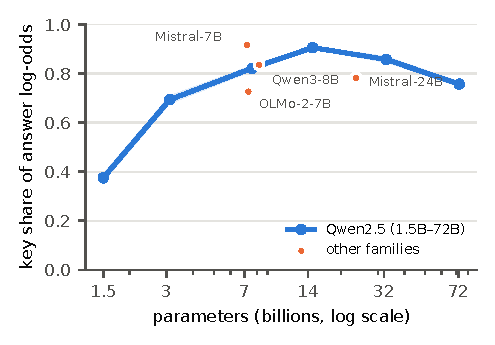
\includegraphics[width=0.55\textwidth]{figures/fig_scale.pdf}
\caption{\textbf{Key share of the \fmtOpt{} answer across scale and families.} $s_K = \bar d_K/(\bar d_K + \bar d_V)$ with keys and values clamped from layer~0. Line and band: Qwen2.5-Instruct 1.5B--72B with 95\% bootstrap CIs; points: other families. $n = 150$ stories per model; values with CIs in \cref{tab:natural}. $s_K$, the preregistered measure, includes non-specific effects; the identity key share $s_{\mathrm{ID}}$ shows the same rise to 14B and fall beyond (\cref{tab:idshare}). Exploratory (B3), with the threshold of C4.}
\label{fig:scale}
\end{figure}

\paragraph{Identity key share.} \Cref{tab:idshare} normalises $\mathrm{ID}_K$ by the total identity effect, $s_{\mathrm{ID}} = \overline{\mathrm{ID}}_K/(\overline{\mathrm{ID}}_K + \overline{\mathrm{ID}}_V)$, so that formats and models with different confidence can be compared. It tracks $s_K$ closely except under \fmtNone{} and \fmtBefore{}, where $s_K$ also counts the non-specific effect of a foreign key. Above 1.5B it is \idShareLetterMinNoOnefive{}--\idShareLetterMax{} under \fmtLetter{} and at most \idShareBeforeMax{} under \fmtBefore{} (exploratory); the table gives the other formats.

\begin{table}[!ht]
\centering
\small
\caption{\textbf{Identity key share $s_{\mathrm{ID}}$, all models} (exploratory). Ratio of mean $\mathrm{ID}_K$ to mean $\mathrm{ID}_K + \mathrm{ID}_V$, keys and values clamped from layer~0; $n = 150$ stories per format and model; 95\% bootstrap CIs, ratio recomputed in each resample.}
\label{tab:idshare}
\begin{tabular}{lccccc}
\toprule
Model & \fmtLetter & \fmtOpt & \fmtPost & \fmtNone & \fmtBefore \\
\midrule
Qwen2.5-1.5B & \begin{tabular}[t]{@{}c@{}}+0.83\\[-1pt]{\scriptsize[+0.81, +0.86]}\end{tabular} & \begin{tabular}[t]{@{}c@{}}+0.36\\[-1pt]{\scriptsize[+0.34, +0.38]}\end{tabular} & \begin{tabular}[t]{@{}c@{}}-0.08\\[-1pt]{\scriptsize[-0.10, -0.06]}\end{tabular} & \begin{tabular}[t]{@{}c@{}}+0.02\\[-1pt]{\scriptsize[+0.01, +0.02]}\end{tabular} & \begin{tabular}[t]{@{}c@{}}-0.04\\[-1pt]{\scriptsize[-0.05, -0.03]}\end{tabular} \\
Qwen2.5-3B & \begin{tabular}[t]{@{}c@{}}+0.98\\[-1pt]{\scriptsize[+0.97, +0.99]}\end{tabular} & \begin{tabular}[t]{@{}c@{}}+0.67\\[-1pt]{\scriptsize[+0.66, +0.69]}\end{tabular} & \begin{tabular}[t]{@{}c@{}}-0.00\\[-1pt]{\scriptsize[-0.04, +0.03]}\end{tabular} & \begin{tabular}[t]{@{}c@{}}+0.00\\[-1pt]{\scriptsize[-0.00, +0.01]}\end{tabular} & \begin{tabular}[t]{@{}c@{}}-0.05\\[-1pt]{\scriptsize[-0.06, -0.04]}\end{tabular} \\
Mistral-7B & \begin{tabular}[t]{@{}c@{}}+0.94\\[-1pt]{\scriptsize[+0.92, +0.95]}\end{tabular} & \begin{tabular}[t]{@{}c@{}}+0.87\\[-1pt]{\scriptsize[+0.85, +0.88]}\end{tabular} & \begin{tabular}[t]{@{}c@{}}+0.41\\[-1pt]{\scriptsize[+0.39, +0.43]}\end{tabular} & \begin{tabular}[t]{@{}c@{}}+0.04\\[-1pt]{\scriptsize[+0.03, +0.04]}\end{tabular} & \begin{tabular}[t]{@{}c@{}}+0.00\\[-1pt]{\scriptsize[-0.00, +0.00]}\end{tabular} \\
OLMo-2-7B & \begin{tabular}[t]{@{}c@{}}+0.99\\[-1pt]{\scriptsize[+0.99, +0.99]}\end{tabular} & \begin{tabular}[t]{@{}c@{}}+0.69\\[-1pt]{\scriptsize[+0.68, +0.70]}\end{tabular} & \begin{tabular}[t]{@{}c@{}}+0.19\\[-1pt]{\scriptsize[+0.17, +0.20]}\end{tabular} & \begin{tabular}[t]{@{}c@{}}+0.03\\[-1pt]{\scriptsize[+0.03, +0.04]}\end{tabular} & \begin{tabular}[t]{@{}c@{}}-0.03\\[-1pt]{\scriptsize[-0.03, -0.02]}\end{tabular} \\
Qwen2.5-7B & \begin{tabular}[t]{@{}c@{}}+0.99\\[-1pt]{\scriptsize[+0.98, +0.99]}\end{tabular} & \begin{tabular}[t]{@{}c@{}}+0.79\\[-1pt]{\scriptsize[+0.77, +0.80]}\end{tabular} & \begin{tabular}[t]{@{}c@{}}+0.32\\[-1pt]{\scriptsize[+0.30, +0.33]}\end{tabular} & \begin{tabular}[t]{@{}c@{}}+0.06\\[-1pt]{\scriptsize[+0.05, +0.06]}\end{tabular} & \begin{tabular}[t]{@{}c@{}}-0.01\\[-1pt]{\scriptsize[-0.01, -0.00]}\end{tabular} \\
Qwen3-8B & \begin{tabular}[t]{@{}c@{}}+0.97\\[-1pt]{\scriptsize[+0.97, +0.98]}\end{tabular} & \begin{tabular}[t]{@{}c@{}}+0.81\\[-1pt]{\scriptsize[+0.80, +0.82]}\end{tabular} & \begin{tabular}[t]{@{}c@{}}+0.29\\[-1pt]{\scriptsize[+0.28, +0.30]}\end{tabular} & \begin{tabular}[t]{@{}c@{}}+0.05\\[-1pt]{\scriptsize[+0.04, +0.05]}\end{tabular} & \begin{tabular}[t]{@{}c@{}}-0.01\\[-1pt]{\scriptsize[-0.02, -0.01]}\end{tabular} \\
Qwen2.5-14B & \begin{tabular}[t]{@{}c@{}}+1.00\\[-1pt]{\scriptsize[+1.00, +1.00]}\end{tabular} & \begin{tabular}[t]{@{}c@{}}+0.88\\[-1pt]{\scriptsize[+0.87, +0.89]}\end{tabular} & \begin{tabular}[t]{@{}c@{}}+0.40\\[-1pt]{\scriptsize[+0.38, +0.41]}\end{tabular} & \begin{tabular}[t]{@{}c@{}}+0.05\\[-1pt]{\scriptsize[+0.05, +0.06]}\end{tabular} & \begin{tabular}[t]{@{}c@{}}-0.00\\[-1pt]{\scriptsize[-0.01, -0.00]}\end{tabular} \\
Mistral-24B & \begin{tabular}[t]{@{}c@{}}+0.98\\[-1pt]{\scriptsize[+0.98, +0.98]}\end{tabular} & \begin{tabular}[t]{@{}c@{}}+0.73\\[-1pt]{\scriptsize[+0.72, +0.74]}\end{tabular} & \begin{tabular}[t]{@{}c@{}}+0.45\\[-1pt]{\scriptsize[+0.44, +0.46]}\end{tabular} & \begin{tabular}[t]{@{}c@{}}+0.04\\[-1pt]{\scriptsize[+0.03, +0.05]}\end{tabular} & \begin{tabular}[t]{@{}c@{}}-0.06\\[-1pt]{\scriptsize[-0.07, -0.05]}\end{tabular} \\
Qwen2.5-32B & \begin{tabular}[t]{@{}c@{}}+0.99\\[-1pt]{\scriptsize[+0.99, +0.99]}\end{tabular} & \begin{tabular}[t]{@{}c@{}}+0.82\\[-1pt]{\scriptsize[+0.81, +0.83]}\end{tabular} & \begin{tabular}[t]{@{}c@{}}+0.30\\[-1pt]{\scriptsize[+0.29, +0.32]}\end{tabular} & \begin{tabular}[t]{@{}c@{}}+0.04\\[-1pt]{\scriptsize[+0.04, +0.05]}\end{tabular} & \begin{tabular}[t]{@{}c@{}}-0.01\\[-1pt]{\scriptsize[-0.02, -0.01]}\end{tabular} \\
Qwen2.5-72B & \begin{tabular}[t]{@{}c@{}}+0.99\\[-1pt]{\scriptsize[+0.99, +0.99]}\end{tabular} & \begin{tabular}[t]{@{}c@{}}+0.71\\[-1pt]{\scriptsize[+0.70, +0.72]}\end{tabular} & \begin{tabular}[t]{@{}c@{}}+0.33\\[-1pt]{\scriptsize[+0.31, +0.34]}\end{tabular} & \begin{tabular}[t]{@{}c@{}}+0.02\\[-1pt]{\scriptsize[+0.02, +0.02]}\end{tabular} & \begin{tabular}[t]{@{}c@{}}-0.09\\[-1pt]{\scriptsize[-0.10, -0.08]}\end{tabular} \\
\bottomrule
\end{tabular}

\end{table}

\begin{figure}[!ht]
\centering
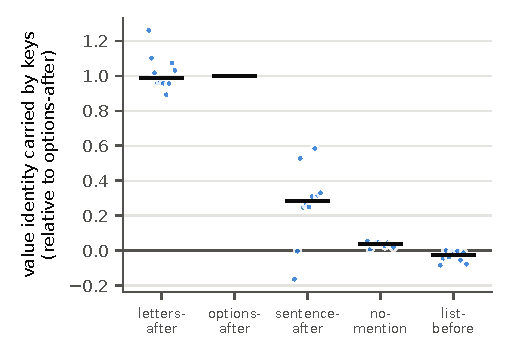
\includegraphics[width=0.55\textwidth]{figures/fig_formats.pdf}
\caption{\textbf{Key identity by format, relative to \fmtOpt{}.} Each point is one of the \nModels{} models: $\mathrm{ID}_K$ in that format divided by $\mathrm{ID}_K$ under \fmtOpt{} in the same model (so \fmtOpt{} is 1 by construction); points are jittered horizontally, and the horizontal line is the median over models. $n = 150$ stories per format and model; per-model values with 95\% bootstrap CIs are in \cref{tab:natural}.}
\label{fig:formats}
\end{figure}

\paragraph{Decomposition.} \Cref{tab:decomposition} gives, for each model and format, the effects of clamping the key, the value or both, the interaction $d_{KV} - d_K - d_V$, and $\mathrm{ID}_V$. The interaction is small relative to $d_{KV}$ in every cell, so the two channels' effects add up. Under \fmtLetter{} the value channel carries almost no identity in any model, and under \fmtNone{} and \fmtBefore{} it carries most of it: there the identity is copied. In the instruction-matched $2{\times}2$ (\cref{tab:twobytwo}), $\mathrm{ID}_K$ is larger under \fmtListA{} than under \fmtPost{} in all four models, and \fmtListA{} is close to \fmtOpt{} in the same model; neither comparison was preregistered.

\begin{table}[!ht]
\centering
\footnotesize
\caption{\textbf{Key/value decomposition.} Mean effects (nats of $m_{\mathrm{SB}}$) of clamping the writing token's key ($d_K$), value ($d_V$) or both ($d_{KV}$) to the source run's from layer~0, measured against the self-clamp row; the interaction $d_{KV} - d_K - d_V$ with its 95\% bootstrap CI; and the value identity $\mathrm{ID}_V$ (nats). $n = 150$ stories per format and model.}
\label{tab:decomposition}
\begin{tabular}{llrrrrr}
\toprule
Model & Format & $d_K$ & $d_V$ & $d_{KV}$ & interaction & $\mathrm{ID}_V$ \\
\midrule
Qwen2.5-1.5B & letters- after & +9.9 & +4.2 & +14.5 & +0.4 \tiny[-0.5, +1.3] & +0.7 \\
 & options- after & +6.3 & +10.4 & +16.7 & -0.0 \tiny[-0.5, +0.5] & +5.0 \\
 & sentence- after & +0.5 & +14.4 & +14.8 & -0.0 \tiny[-0.4, +0.3] & +6.5 \\
 & no- mention & +1.8 & +21.8 & +23.5 & -0.1 \tiny[-0.7, +0.5] & +10.2 \\
 & list- before & +1.2 & +13.6 & +14.5 & -0.3 \tiny[-0.6, +0.1] & +5.9 \\
\midrule
Qwen2.5-3B & letters- after & +22.3 & +0.8 & +22.8 & -0.4 \tiny[-1.1, +0.3] & +0.2 \\
 & options- after & +20.4 & +9.0 & +29.1 & -0.4 \tiny[-1.1, +0.3] & +5.0 \\
 & sentence- after & +2.9 & +26.8 & +29.9 & +0.2 \tiny[-0.6, +1.0] & +11.8 \\
 & no- mention & +4.3 & +41.1 & +45.9 & +0.5 \tiny[-0.1, +1.1] & +18.1 \\
 & list- before & +2.8 & +23.4 & +26.4 & +0.2 \tiny[-0.5, +0.8] & +9.6 \\
\midrule
Mistral-7B & letters- after & +31.3 & +1.5 & +32.2 & -0.5 \tiny[-1.2, +0.1] & +1.0 \\
 & options- after & +28.0 & +2.6 & +30.8 & +0.1 \tiny[-0.6, +0.8] & +2.3 \\
 & sentence- after & +12.9 & +19.5 & +31.8 & -0.6 \tiny[-2.3, +1.1] & +11.5 \\
 & no- mention & +2.7 & +28.8 & +31.5 & -0.1 \tiny[-0.4, +0.3] & +13.6 \\
 & list- before & +1.2 & +30.9 & +32.1 & +0.1 \tiny[-0.3, +0.5] & +14.6 \\
\midrule
OLMo-2-7B & letters- after & +15.6 & +0.1 & +15.7 & +0.0 \tiny[-0.1, +0.1] & +0.1 \\
 & options- after & +15.5 & +5.8 & +21.0 & -0.3 \tiny[-0.9, +0.2] & +3.7 \\
 & sentence- after & +3.8 & +16.8 & +20.7 & +0.0 \tiny[-0.5, +0.6] & +8.6 \\
 & no- mention & +2.7 & +23.5 & +26.1 & -0.1 \tiny[-0.5, +0.3] & +11.0 \\
 & list- before & +0.2 & +23.6 & +23.9 & +0.1 \tiny[-0.1, +0.4] & +11.2 \\
\midrule
Qwen2.5-7B & letters- after & +40.2 & +1.1 & +41.2 & -0.1 \tiny[-0.7, +0.4] & +0.2 \\
 & options- after & +39.6 & +8.6 & +47.9 & -0.4 \tiny[-1.1, +0.3] & +5.8 \\
 & sentence- after & +11.0 & +23.1 & +34.4 & +0.4 \tiny[-0.4, +1.1] & +11.9 \\
 & no- mention & +6.0 & +36.8 & +42.5 & -0.3 \tiny[-0.7, +0.2] & +16.6 \\
 & list- before & +2.4 & +34.8 & +36.8 & -0.4 \tiny[-0.8, -0.1] & +16.0 \\
\midrule
Qwen3-8B & letters- after & +66.8 & +1.2 & +67.9 & -0.1 \tiny[-0.5, +0.3] & +1.0 \\
 & options- after & +67.1 & +13.2 & +80.5 & +0.2 \tiny[-1.4, +1.7] & +8.2 \\
 & sentence- after & +14.3 & +40.0 & +53.3 & -1.1 \tiny[-2.5, +0.3] & +21.8 \\
 & no- mention & +5.7 & +54.4 & +59.4 & -0.7 \tiny[-1.6, +0.2] & +25.3 \\
 & list- before & +2.9 & +51.8 & +54.4 & -0.3 \tiny[-0.8, +0.2] & +24.0 \\
\midrule
Qwen2.5-14B & letters- after & +70.0 & +0.2 & +70.2 & +0.0 \tiny[-0.2, +0.3] & +0.1 \\
 & options- after & +75.0 & +7.8 & +82.8 & -0.1 \tiny[-0.7, +0.5] & +5.4 \\
 & sentence- after & +21.9 & +33.8 & +56.9 & +1.1 \tiny[-1.4, +3.6] & +18.5 \\
 & no- mention & +10.8 & +46.5 & +57.1 & -0.2 \tiny[-0.9, +0.4] & +19.1 \\
 & list- before & +2.4 & +65.9 & +68.3 & +0.0 \tiny[-0.5, +0.5] & +31.1 \\
\midrule
Mistral-24B & letters- after & +18.7 & +0.4 & +19.0 & -0.1 \tiny[-0.2, -0.0] & +0.2 \\
 & options- after & +17.1 & +4.8 & +21.9 & +0.1 \tiny[-0.2, +0.4] & +3.6 \\
 & sentence- after & +8.1 & +10.4 & +18.6 & +0.1 \tiny[-0.7, +0.8] & +6.8 \\
 & no- mention & +2.0 & +20.8 & +22.6 & -0.2 \tiny[-0.4, +0.0] & +9.8 \\
 & list- before & -0.0 & +19.4 & +19.4 & +0.1 \tiny[-0.1, +0.3] & +9.1 \\
\midrule
Qwen2.5-32B & letters- after & +69.5 & +0.6 & +70.3 & +0.2 \tiny[-0.1, +0.5] & +0.3 \\
 & options- after & +61.4 & +10.2 & +71.6 & -0.1 \tiny[-1.8, +1.7] & +7.1 \\
 & sentence- after & +18.7 & +44.8 & +63.1 & -0.4 \tiny[-2.0, +1.3] & +23.4 \\
 & no- mention & +9.8 & +53.8 & +63.4 & -0.2 \tiny[-0.9, +0.5] & +23.4 \\
 & list- before & +2.8 & +65.1 & +68.1 & +0.1 \tiny[-0.5, +0.7] & +30.6 \\
\midrule
Qwen2.5-72B & letters- after & +52.8 & +0.2 & +53.0 & -0.0 \tiny[-0.2, +0.2] & +0.3 \\
 & options- after & +44.6 & +14.3 & +59.6 & +0.7 \tiny[-0.3, +1.7] & +10.5 \\
 & sentence- after & +14.4 & +30.9 & +46.4 & +1.1 \tiny[-0.3, +2.6] & +17.5 \\
 & no- mention & +3.1 & +47.7 & +50.9 & +0.1 \tiny[-0.4, +0.5] & +22.9 \\
 & list- before & -1.7 & +51.2 & +49.8 & +0.3 \tiny[-0.2, +0.7] & +24.1 \\
\bottomrule
\end{tabular}

\end{table}

\paragraph{Clamp onset.} Layer-0 keys are a function of the input embedding alone, so \cref{tab:onset} starts both clamps deeper (exploratory). With $\ell_0 \approx 0.06L$ the shares are essentially unchanged in eight of ten models. With $\ell_0 \approx 0.3L$ the share stays at or above one half in seven models (up to \onsetLateQwenFourteen{} at Qwen2.5-14B), but falls to \onsetLateQwenOnefive{} at Qwen2.5-1.5B, \onsetLateMistralTwentyfour{} at Mistral-Small-24B and \onsetLateOlmoSeven{} at OLMo-2-7B, where the key effect depends on the lowest layers. Deeper keys therefore still carry the written word in most models. With $\ell_0 > 0$ the clamp is no longer exact, and at $\ell_0 \approx 0.3L$ the key and value effects no longer add up: the interaction is positive in every model (result summaries). The share at that onset is therefore descriptive only.

\begin{table}[!ht]
\centering
\caption{\textbf{Key share by clamp onset.} $s_K = \bar d_K / (\bar d_K + \bar d_V)$ under \fmtOpt{} with both clamps applied from layer $\ell_0$ on; the onset used in each model is given in brackets. $n = 150$ stories per model; point estimates (the $\ell_0 = 0$ intervals are in \cref{tab:natural}). Exploratory.}
\label{tab:onset}
\begin{tabular}{lcccc}
\toprule
Model & layers $L$ & $s_K$, onset $\ell_0{=}0$ & $s_K$, $\ell_0{\approx}0.06L$ & $s_K$, $\ell_0{\approx}0.3L$ \\
\midrule
Qwen2.5-1.5B & 28 & 0.37 ($\ell_0{=}0$) & 0.37 ($\ell_0{=}2$) & 0.19 ($\ell_0{=}8$) \\
Qwen2.5-3B & 36 & 0.69 ($\ell_0{=}0$) & 0.69 ($\ell_0{=}2$) & 0.56 ($\ell_0{=}11$) \\
Mistral-7B & 32 & 0.92 ($\ell_0{=}0$) & 0.91 ($\ell_0{=}2$) & 0.53 ($\ell_0{=}10$) \\
OLMo-2-7B & 32 & 0.73 ($\ell_0{=}0$) & 0.72 ($\ell_0{=}2$) & 0.03 ($\ell_0{=}10$) \\
Qwen2.5-7B & 28 & 0.82 ($\ell_0{=}0$) & 0.82 ($\ell_0{=}2$) & 0.66 ($\ell_0{=}8$) \\
Qwen3-8B & 36 & 0.84 ($\ell_0{=}0$) & 0.84 ($\ell_0{=}2$) & 0.73 ($\ell_0{=}11$) \\
Qwen2.5-14B & 48 & 0.91 ($\ell_0{=}0$) & 0.91 ($\ell_0{=}3$) & 0.83 ($\ell_0{=}14$) \\
Mistral-24B & 40 & 0.78 ($\ell_0{=}0$) & 0.78 ($\ell_0{=}2$) & 0.37 ($\ell_0{=}12$) \\
Qwen2.5-32B & 64 & 0.86 ($\ell_0{=}0$) & 0.86 ($\ell_0{=}4$) & 0.82 ($\ell_0{=}19$) \\
Qwen2.5-72B & 80 & 0.76 ($\ell_0{=}0$) & 0.76 ($\ell_0{=}5$) & 0.55 ($\ell_0{=}24$) \\
\bottomrule
\end{tabular}

\end{table}

\paragraph{Layer windows and KV groups.} \Cref{tab:windows} refines the row-restricted splice at Qwen2.5-1.5B (28 layers, two KV groups). Only the option-word rows see the source key, and the swap is further limited to a window of four layers (all KV groups) or to one KV group's slice of the key (all layers). The read happens in layers 4--15, and KV group 1 carries more of it than KV group 0 in both formats. The seven windows together recover less than the option-word rows do with the swap at all layers, and the two single-group swaps together recover less than both groups at once, so the read compounds across layers and groups. We ran the same window and KV-group splices, on the option-word rows under \fmtOpt{} and \fmtLetter{}, at Qwen2.5-7B, Qwen2.5-14B and Mistral-7B (exploratory; result summaries). In these models no single four-layer window and no single KV group recovers most of the option-word effect, so the dominance of one KV group seen at 1.5B does not carry over.

\begin{table}[!ht]
\centering
\caption{\textbf{Depth and KV-group localisation of the option-word key read} (Qwen2.5-1.5B, FP32). Entries are fractions of the effect obtained when the option-word rows see the source key in every layer and both KV groups, with 95\% bootstrap CIs over stories (ratio of means recomputed in each resample). $n = 40$ stories per format. Exploratory.}
\label{tab:windows}
\begin{tabular}{lcc}
\toprule
Rows/layers that see the swapped key & \fmtOpt & \fmtLetter \\
\midrule
layers 0--3 & $-$0.02 \tiny[$-$0.02, $-$0.01] & $-$0.01 \tiny[$-$0.01, 0.00] \\
layers 4--7 & +0.23 \tiny[+0.11, +0.35] & +0.36 \tiny[+0.26, +0.46] \\
layers 8--11 & +0.14 \tiny[+0.10, +0.18] & +0.06 \tiny[+0.03, +0.09] \\
layers 12--15 & +0.15 \tiny[+0.12, +0.19] & +0.04 \tiny[+0.02, +0.06] \\
layers 16--19 & +0.02 \tiny[+0.01, +0.04] & +0.01 \tiny[0.00, +0.02] \\
layers 20--23 & 0.00 \tiny[0.00, 0.00] & 0.00 \tiny[0.00, 0.00] \\
layers 24--27 & 0.00 \tiny[0.00, 0.00] & 0.00 \tiny[0.00, 0.00] \\
KV group 0 (all layers) & +0.22 \tiny[+0.17, +0.27] & +0.06 \tiny[+0.03, +0.09] \\
KV group 1 (all layers) & +0.53 \tiny[+0.40, +0.66] & +0.66 \tiny[+0.57, +0.75] \\
\bottomrule
\end{tabular}

\end{table}

\paragraph{New tasks.} \Cref{tab:tasks} gives the paint and schedule results. In every model and both tasks, $\mathrm{ID}_K$ is large under \fmtLetter{} and \fmtOpt{}, intermediate under \fmtPost{}, small under \fmtNone{} and near zero under \fmtBefore{}. The \fmtOpt{} key share ranges from \taskPaintShareMin{} to \taskPaintShareMax{} (paint) and from \taskScheduleShareMin{} to \taskScheduleShareMax{} (schedule), lowest at OLMo-2-7B in both.

\begin{table}[!ht]
\centering
\caption{\textbf{Paint and schedule tasks.} Key share under \fmtOpt{} and $\mathrm{ID}_K$ (nats) in each format, clamped from layer~0. $n = 150$ stories per task, format and model; 95\% bootstrap CIs. Preregistration D (D1, D2) for \fmtOpt{}, \fmtNone{} and \fmtBefore{}; the rest exploratory.}
\label{tab:tasks}
\resizebox{\textwidth}{!}{\begin{tabular}{llcccccc}
\toprule
Task & Model & $s_K$ (\fmtOpt) & \multicolumn{5}{c}{$\mathrm{ID}_K$ (nats)} \\
\cmidrule(lr){4-8}
 & & & \fmtLetter & \fmtOpt & \fmtPost & \fmtNone & \fmtBefore \\
\midrule
paint & Qwen2.5-7B & \begin{tabular}[t]{@{}c@{}}0.73\\[-1pt]{\scriptsize[0.72, 0.74]}\end{tabular} & \begin{tabular}[t]{@{}c@{}}+21.5\\[-1pt]{\scriptsize[+21.3, +21.7]}\end{tabular} & \begin{tabular}[t]{@{}c@{}}+21.4\\[-1pt]{\scriptsize[+21.2, +21.7]}\end{tabular} & \begin{tabular}[t]{@{}c@{}}+3.0\\[-1pt]{\scriptsize[+2.8, +3.1]}\end{tabular} & \begin{tabular}[t]{@{}c@{}}+1.2\\[-1pt]{\scriptsize[+1.1, +1.3]}\end{tabular} & \begin{tabular}[t]{@{}c@{}}+0.3\\[-1pt]{\scriptsize[+0.2, +0.4]}\end{tabular} \\
 & Qwen2.5-14B & \begin{tabular}[t]{@{}c@{}}0.90\\[-1pt]{\scriptsize[0.90, 0.91]}\end{tabular} & \begin{tabular}[t]{@{}c@{}}+35.7\\[-1pt]{\scriptsize[+35.4, +36.0]}\end{tabular} & \begin{tabular}[t]{@{}c@{}}+40.3\\[-1pt]{\scriptsize[+39.9, +40.8]}\end{tabular} & \begin{tabular}[t]{@{}c@{}}+3.5\\[-1pt]{\scriptsize[+3.3, +3.7]}\end{tabular} & \begin{tabular}[t]{@{}c@{}}+0.8\\[-1pt]{\scriptsize[+0.7, +0.9]}\end{tabular} & \begin{tabular}[t]{@{}c@{}}+0.2\\[-1pt]{\scriptsize[+0.1, +0.2]}\end{tabular} \\
 & Qwen3-8B & \begin{tabular}[t]{@{}c@{}}0.92\\[-1pt]{\scriptsize[0.92, 0.93]}\end{tabular} & \begin{tabular}[t]{@{}c@{}}+39.7\\[-1pt]{\scriptsize[+39.4, +40.1]}\end{tabular} & \begin{tabular}[t]{@{}c@{}}+42.7\\[-1pt]{\scriptsize[+42.3, +43.0]}\end{tabular} & \begin{tabular}[t]{@{}c@{}}+4.9\\[-1pt]{\scriptsize[+4.7, +5.2]}\end{tabular} & \begin{tabular}[t]{@{}c@{}}+1.1\\[-1pt]{\scriptsize[+1.0, +1.2]}\end{tabular} & \begin{tabular}[t]{@{}c@{}}+0.1\\[-1pt]{\scriptsize[+0.1, +0.2]}\end{tabular} \\
 & Mistral-7B & \begin{tabular}[t]{@{}c@{}}0.86\\[-1pt]{\scriptsize[0.85, 0.87]}\end{tabular} & \begin{tabular}[t]{@{}c@{}}+16.0\\[-1pt]{\scriptsize[+15.7, +16.3]}\end{tabular} & \begin{tabular}[t]{@{}c@{}}+16.1\\[-1pt]{\scriptsize[+15.9, +16.4]}\end{tabular} & \begin{tabular}[t]{@{}c@{}}+2.2\\[-1pt]{\scriptsize[+1.9, +2.4]}\end{tabular} & \begin{tabular}[t]{@{}c@{}}+0.4\\[-1pt]{\scriptsize[+0.3, +0.5]}\end{tabular} & \begin{tabular}[t]{@{}c@{}}+0.1\\[-1pt]{\scriptsize[+0.1, +0.2]}\end{tabular} \\
 & OLMo-2-7B & \begin{tabular}[t]{@{}c@{}}0.47\\[-1pt]{\scriptsize[0.46, 0.48]}\end{tabular} & \begin{tabular}[t]{@{}c@{}}+7.4\\[-1pt]{\scriptsize[+7.2, +7.5]}\end{tabular} & \begin{tabular}[t]{@{}c@{}}+6.5\\[-1pt]{\scriptsize[+6.3, +6.7]}\end{tabular} & \begin{tabular}[t]{@{}c@{}}+0.7\\[-1pt]{\scriptsize[+0.6, +0.8]}\end{tabular} & \begin{tabular}[t]{@{}c@{}}+0.1\\[-1pt]{\scriptsize[+0.1, +0.2]}\end{tabular} & \begin{tabular}[t]{@{}c@{}}-0.1\\[-1pt]{\scriptsize[-0.1, -0.1]}\end{tabular} \\
\midrule
schedule & Qwen2.5-7B & \begin{tabular}[t]{@{}c@{}}0.58\\[-1pt]{\scriptsize[0.56, 0.59]}\end{tabular} & \begin{tabular}[t]{@{}c@{}}+19.6\\[-1pt]{\scriptsize[+19.3, +20.0]}\end{tabular} & \begin{tabular}[t]{@{}c@{}}+12.7\\[-1pt]{\scriptsize[+12.4, +13.0]}\end{tabular} & \begin{tabular}[t]{@{}c@{}}+4.1\\[-1pt]{\scriptsize[+3.8, +4.4]}\end{tabular} & \begin{tabular}[t]{@{}c@{}}+0.1\\[-1pt]{\scriptsize[+0.1, +0.2]}\end{tabular} & \begin{tabular}[t]{@{}c@{}}-0.1\\[-1pt]{\scriptsize[-0.2, -0.1]}\end{tabular} \\
 & Qwen2.5-14B & \begin{tabular}[t]{@{}c@{}}0.87\\[-1pt]{\scriptsize[0.87, 0.88]}\end{tabular} & \begin{tabular}[t]{@{}c@{}}+35.6\\[-1pt]{\scriptsize[+35.3, +35.9]}\end{tabular} & \begin{tabular}[t]{@{}c@{}}+26.1\\[-1pt]{\scriptsize[+25.7, +26.5]}\end{tabular} & \begin{tabular}[t]{@{}c@{}}+10.9\\[-1pt]{\scriptsize[+10.3, +11.6]}\end{tabular} & \begin{tabular}[t]{@{}c@{}}+0.6\\[-1pt]{\scriptsize[+0.5, +0.6]}\end{tabular} & \begin{tabular}[t]{@{}c@{}}+0.2\\[-1pt]{\scriptsize[+0.1, +0.2]}\end{tabular} \\
 & Qwen3-8B & \begin{tabular}[t]{@{}c@{}}0.92\\[-1pt]{\scriptsize[0.91, 0.92]}\end{tabular} & \begin{tabular}[t]{@{}c@{}}+39.6\\[-1pt]{\scriptsize[+39.2, +40.0]}\end{tabular} & \begin{tabular}[t]{@{}c@{}}+28.5\\[-1pt]{\scriptsize[+28.0, +29.0]}\end{tabular} & \begin{tabular}[t]{@{}c@{}}+7.3\\[-1pt]{\scriptsize[+6.9, +7.7]}\end{tabular} & \begin{tabular}[t]{@{}c@{}}+0.9\\[-1pt]{\scriptsize[+0.8, +1.0]}\end{tabular} & \begin{tabular}[t]{@{}c@{}}+0.2\\[-1pt]{\scriptsize[+0.1, +0.2]}\end{tabular} \\
 & Mistral-7B & \begin{tabular}[t]{@{}c@{}}0.82\\[-1pt]{\scriptsize[0.81, 0.84]}\end{tabular} & \begin{tabular}[t]{@{}c@{}}+16.2\\[-1pt]{\scriptsize[+15.6, +16.7]}\end{tabular} & \begin{tabular}[t]{@{}c@{}}+13.2\\[-1pt]{\scriptsize[+12.9, +13.5]}\end{tabular} & \begin{tabular}[t]{@{}c@{}}+5.1\\[-1pt]{\scriptsize[+4.6, +5.6]}\end{tabular} & \begin{tabular}[t]{@{}c@{}}+0.1\\[-1pt]{\scriptsize[+0.1, +0.2]}\end{tabular} & \begin{tabular}[t]{@{}c@{}}-0.0\\[-1pt]{\scriptsize[-0.1, +0.0]}\end{tabular} \\
 & OLMo-2-7B & \begin{tabular}[t]{@{}c@{}}0.35\\[-1pt]{\scriptsize[0.34, 0.37]}\end{tabular} & \begin{tabular}[t]{@{}c@{}}+7.4\\[-1pt]{\scriptsize[+7.2, +7.6]}\end{tabular} & \begin{tabular}[t]{@{}c@{}}+4.5\\[-1pt]{\scriptsize[+4.3, +4.7]}\end{tabular} & \begin{tabular}[t]{@{}c@{}}+2.3\\[-1pt]{\scriptsize[+2.1, +2.4]}\end{tabular} & \begin{tabular}[t]{@{}c@{}}+0.1\\[-1pt]{\scriptsize[+0.1, +0.1]}\end{tabular} & \begin{tabular}[t]{@{}c@{}}+0.0\\[-1pt]{\scriptsize[-0.0, +0.1]}\end{tabular} \\
\bottomrule
\end{tabular}
}
\end{table}

\paragraph{Role control.} Could the writing token's channels carry more than identity, such as whether the person asked about saw the move? The role-swap control exchanges the observer's and the non-observer's names but keeps the location word (\cref{app:prompts}). \Cref{tab:role} gives the role-swap effect and the fractions of it that the writing token's key and value carry. The swap shifts the belief answer by \roleEffMin{} to \roleEffMax{} nats, depending on model and format, and clamping either channel alone to the role-swapped run carries at most \roleFracMax{} of that shift, under \fmtOpt{}, \fmtNone{} and \fmtLetter{}, in five models including Qwen2.5-72B. The prediction was preregistered for \fmtOpt{} and \fmtNone{} in four models, with a bound of 0.15 (E2, met); \fmtLetter{} and Qwen2.5-72B are exploratory. The writing token's key and value thus carry \emph{which} value was written, not the observer's name; an ordering-ID address of the observer, the same in both runs, would not register (\cref{app:discussion}).

\begin{table}[!ht]
\centering
\caption{\textbf{Identity, not belief role.} Role effect: mean change in $m = \log p(\text{initial}) - \log p(\textsc{loc})$ when the observer and non-observer are swapped with the same location word (nats). $f_K$, $f_V$: fraction of that change reproduced by clamping only the writing token's key or value (all layers) to the role-swapped run's, as a ratio of means. Direct question; $n = 150$ stories per format and model; 95\% bootstrap CIs. Preregistration E (E2) for \fmtOpt{} and \fmtNone{} in the four 7--14B models; \fmtLetter{} and Qwen2.5-72B exploratory.}
\label{tab:role}
\begin{tabular}{llccc}
\toprule
Model & Format & role effect (nats) & $f_K$ & $f_V$ \\
\midrule
Qwen2.5-7B & options- after & +34.4 & +0.006 & +0.010 \\
 & no- mention & +28.7 & +0.014 & +0.001 \\
 & letters- after & +29.8 & +0.003 & +0.018 \\
\midrule
Qwen2.5-14B & options- after & +79.8 & +0.001 & -0.000 \\
 & no- mention & +51.4 & +0.001 & -0.000 \\
 & letters- after & +66.0 & -0.000 & -0.000 \\
\midrule
Mistral-7B & options- after & +28.4 & +0.003 & +0.004 \\
 & no- mention & +26.6 & +0.019 & +0.001 \\
 & letters- after & +28.9 & +0.000 & +0.011 \\
\midrule
OLMo-2-7B & options- after & +16.9 & +0.004 & +0.002 \\
 & no- mention & +17.7 & +0.014 & +0.002 \\
 & letters- after & +12.5 & -0.000 & +0.003 \\
\midrule
Qwen2.5-72B & options- after & +50.6 & +0.001 & +0.002 \\
 & no- mention & +38.4 & +0.007 & -0.001 \\
 & letters- after & +46.8 & -0.001 & +0.003 \\
\bottomrule
\end{tabular}

\end{table}

\paragraph{Competent-only analysis.} Our primary analyses pool all stories, whether or not the model answers the clean runs correctly. As a secondary analysis, every natural-factorial quantity is also computed on the stories whose base and source clean runs are both answered correctly (argmax over the candidates). From 7B up most stories are competent and the two analyses agree closely. The competent subset is smallest at Qwen2.5-1.5B and 3B, and the estimates move most at 3B. The sign of $\mathrm{ID}_K$ under \fmtOpt{}, \fmtLetter{}, \fmtNone{} and \fmtBefore{} is unchanged in every model. The near-zero \fmtPost{} value at Qwen2.5-3B becomes slightly positive, with a CI that excludes zero, but stays far below the \fmtPost{} values from 7B up. No conclusion in the main text changes.

\subsection{Fresh stories}\label{app:fresh}

\paragraph{Design.} The fresh stories (\cref{app:prompts-fresh}) were run in eight models: the four discovery-sample models of the instruction-matched $2{\times}2$ (Qwen2.5-7B, Qwen2.5-14B, Mistral-7B, OLMo-2-7B; lines with the suffix P4f, which must hold in every evaluable model, at 95\,\%) and four model families never examined before (Llama-3.1-8B, Gemma-2-9B, Phi-4, Falcon3-7B; lines with the suffix N4, which need three of the four, at 98.75\,\%), plus Gemma-2-2B for the sentence read at small scale. Every statistic uses the emitted-form score (\cref{app:emitted}); its coverage was at least \JbGfourCovMin{} in every cell, so no statistic fell back to its behavioural counterpart. Intervals are two-stage bootstrap intervals over the 55 (lexicon, base, source) cells and the cores within them. They have two limits. For rates at or near 0 or 1 (many $\beta$ cells, and OLMo-2-7B's three flips in 150 stories, where 11.9\,\% of the resamples are exactly zero) percentile intervals are degenerate or unreliable; and with about 2.7 stories per cell, resampling the stories within each drawn cell adds variance, which is conservative for the lines that held but makes near-threshold failures (OLMo-2-7B's sentence read in generated answers) look less certain than they are. Cluster-adjusted exact intervals for these rates were not computed. Generated accuracy on the clean base run was at least \JbGfiveAccMin{} in every arm of the eight models. \Cref{tab:fresh} gives every model and arm. % verbatim: 55 cells, entry J part B

\begin{table}[!ht]
\centering
\footnotesize
\caption{\textbf{Fresh stories, eight models.} 150 fresh cores per model; emitted-form score; 95\,\% two-stage cluster-bootstrap intervals (the N4 lines are decided on 98.75\,\% bounds, given in the text). Arms: AFTER = \fmtListA{}, POST = \fmtPost{}, POST-NULL = \fmtNull{}, PRE = \fmtSentB{}, BEFORE = \fmtBefore{}, NONE = \fmtNone{}. $r$: $\overline{\mathrm{ID}}_K$ in the arm divided by $\overline{\mathrm{ID}}_K$ under AFTER (1 by definition there); $s_{\mathrm{ID}}$: the key share of the value's identity; $\beta_K$, $\beta_V$: the share of generated answers that move to the clamped value under the key-only or value-only clamp, net of moves to it under the clamp to the other of S and X. The first four models are the discovery-sample models (P4), the next four the new families (N4).}
\label{tab:fresh}
{\scriptsize\setlength{\tabcolsep}{5pt}\begin{tabular}{llcccc}
\toprule
Model & Arm & $r$ & $s_{\mathrm{ID}}$ & $\beta_K$ & $\beta_V$ \\
\midrule
Qwen2.5-7B & AFTER & 1 & 0.79 [0.77, 0.81] & 0.99 [0.98, 1.00] & 0.00 [0.00, 0.00] \\
Qwen2.5-7B & POST & 0.27 [0.24, 0.30] & 0.33 [0.30, 0.35] & 0.11 [0.06, 0.16] & 0.86 [0.79, 0.92] \\
Qwen2.5-7B & POST-NULL & 0.03 [0.02, 0.04] & 0.04 [0.03, 0.05] & 0.00 [0.00, 0.00] & 0.92 [0.86, 0.96] \\
Qwen2.5-7B & PRE & -0.01 [-0.02, -0.01] & -0.02 [-0.03, -0.01] & 0.00 [0.00, 0.00] & 1.00 [1.00, 1.00] \\
Qwen2.5-7B & BEFORE & -0.02 [-0.02, -0.01] & -0.02 [-0.03, -0.01] & 0.00 [0.00, 0.00] & 0.96 [0.93, 0.99] \\
Qwen2.5-7B & NONE & 0.03 [0.02, 0.04] & 0.04 [0.03, 0.04] & 0.00 [0.00, 0.00] & 0.97 [0.95, 0.99] \\
\midrule
Qwen2.5-14B & AFTER & 1 & 0.88 [0.86, 0.89] & 1.00 [1.00, 1.00] & 0.00 [0.00, 0.00] \\
Qwen2.5-14B & POST & 0.39 [0.36, 0.43] & 0.39 [0.36, 0.41] & 0.23 [0.16, 0.31] & 0.75 [0.66, 0.83] \\
Qwen2.5-14B & POST-NULL & 0.03 [0.02, 0.04] & 0.05 [0.04, 0.06] & 0.00 [0.00, 0.00] & 0.99 [0.97, 1.00] \\
Qwen2.5-14B & PRE & -0.00 [-0.01, 0.00] & -0.00 [-0.01, 0.00] & 0.00 [0.00, 0.00] & 1.00 [1.00, 1.00] \\
Qwen2.5-14B & BEFORE & -0.00 [-0.01, 0.00] & -0.00 [-0.01, 0.00] & 0.00 [0.00, 0.00] & 1.00 [1.00, 1.00] \\
Qwen2.5-14B & NONE & 0.03 [0.02, 0.04] & 0.05 [0.04, 0.06] & 0.00 [0.00, 0.00] & 0.99 [0.97, 1.00] \\
\midrule
Mistral-7B & AFTER & 1 & 0.80 [0.78, 0.82] & 0.95 [0.91, 0.98] & 0.05 [0.02, 0.09] \\
Mistral-7B & POST & 0.57 [0.50, 0.63] & 0.40 [0.37, 0.43] & 0.31 [0.23, 0.40] & 0.71 [0.62, 0.79] \\
Mistral-7B & POST-NULL & -0.00 [-0.01, 0.01] & -0.00 [-0.01, 0.01] & 0.00 [0.00, 0.00] & 0.93 [0.88, 0.97] \\
Mistral-7B & PRE & -0.03 [-0.05, -0.02] & -0.03 [-0.05, -0.02] & 0.00 [0.00, 0.00] & 0.99 [0.97, 1.00] \\
Mistral-7B & BEFORE & -0.02 [-0.03, -0.01] & -0.02 [-0.03, -0.01] & 0.00 [0.00, 0.00] & 0.98 [0.96, 1.00] \\
Mistral-7B & NONE & -0.00 [-0.01, 0.01] & -0.00 [-0.01, 0.01] & 0.00 [0.00, 0.00] & 0.97 [0.94, 0.99] \\
\midrule
OLMo-2-7B & AFTER & 1 & 0.63 [0.61, 0.65] & 0.86 [0.80, 0.92] & 0.13 [0.07, 0.19] \\
OLMo-2-7B & POST & 0.18 [0.14, 0.22] & 0.16 [0.13, 0.19] & 0.01 [0.00, 0.03] & 0.96 [0.93, 0.99] \\
OLMo-2-7B & POST-NULL & 0.07 [0.05, 0.09] & 0.06 [0.05, 0.07] & 0.00 [0.00, 0.00] & 0.74 [0.66, 0.82] \\
OLMo-2-7B & PRE & -0.05 [-0.07, -0.04] & -0.05 [-0.06, -0.04] & 0.00 [0.00, 0.00] & 1.00 [0.99, 1.00] \\
OLMo-2-7B & BEFORE & -0.04 [-0.06, -0.03] & -0.04 [-0.05, -0.03] & 0.00 [0.00, 0.00] & 1.00 [0.99, 1.00] \\
OLMo-2-7B & NONE & 0.07 [0.05, 0.08] & 0.05 [0.04, 0.06] & 0.00 [0.00, 0.00] & 0.81 [0.74, 0.88] \\
\midrule
Llama-3.1-8B & AFTER & 1 & 0.61 [0.59, 0.63] & 0.76 [0.69, 0.83] & 0.14 [0.08, 0.22] \\
Llama-3.1-8B & POST & 0.40 [0.35, 0.44] & 0.29 [0.26, 0.32] & 0.09 [0.04, 0.13] & 0.88 [0.82, 0.94] \\
Llama-3.1-8B & POST-NULL & 0.12 [0.09, 0.15] & 0.08 [0.06, 0.09] & 0.00 [0.00, 0.00] & 0.90 [0.84, 0.95] \\
Llama-3.1-8B & PRE & -0.03 [-0.05, -0.01] & -0.02 [-0.04, -0.01] & 0.00 [0.00, 0.00] & 1.00 [1.00, 1.00] \\
Llama-3.1-8B & BEFORE & -0.06 [-0.08, -0.05] & -0.05 [-0.07, -0.04] & 0.00 [0.00, 0.00] & 1.00 [1.00, 1.00] \\
Llama-3.1-8B & NONE & 0.11 [0.08, 0.14] & 0.07 [0.06, 0.09] & 0.00 [0.00, 0.00] & 0.88 [0.81, 0.93] \\
\midrule
Gemma-2-9B & AFTER & 1 & 0.70 [0.69, 0.71] & 1.00 [0.99, 1.00] & 0.00 [0.00, 0.00] \\
Gemma-2-9B & POST & 0.51 [0.47, 0.55] & 0.36 [0.34, 0.38] & 0.13 [0.09, 0.19] & 0.84 [0.77, 0.89] \\
Gemma-2-9B & POST-NULL & 0.00 [-0.00, 0.01] & 0.00 [-0.00, 0.01] & 0.00 [0.00, 0.00] & 1.00 [1.00, 1.00] \\
Gemma-2-9B & PRE & -0.02 [-0.03, -0.01] & -0.02 [-0.03, -0.02] & 0.00 [0.00, 0.00] & 1.00 [1.00, 1.00] \\
Gemma-2-9B & BEFORE & -0.02 [-0.02, -0.01] & -0.02 [-0.03, -0.02] & 0.00 [0.00, 0.00] & 1.00 [1.00, 1.00] \\
Gemma-2-9B & NONE & 0.01 [-0.00, 0.01] & 0.00 [-0.00, 0.01] & 0.00 [0.00, 0.00] & 1.00 [1.00, 1.00] \\
\midrule
Phi-4 & AFTER & 1 & 0.72 [0.71, 0.74] & 0.99 [0.97, 1.00] & 0.02 [0.00, 0.04] \\
Phi-4 & POST & 0.33 [0.30, 0.37] & 0.28 [0.26, 0.30] & 0.03 [0.01, 0.06] & 0.97 [0.94, 0.99] \\
Phi-4 & POST-NULL & 0.00 [-0.01, 0.01] & 0.00 [-0.01, 0.01] & 0.00 [0.00, 0.00] & 0.97 [0.92, 1.00] \\
Phi-4 & PRE & -0.03 [-0.03, -0.02] & -0.03 [-0.03, -0.02] & 0.00 [0.00, 0.00] & 1.00 [1.00, 1.00] \\
Phi-4 & BEFORE & -0.05 [-0.05, -0.04] & -0.06 [-0.08, -0.05] & 0.00 [0.00, 0.00] & 0.96 [0.92, 0.99] \\
Phi-4 & NONE & 0.01 [-0.00, 0.02] & 0.01 [-0.00, 0.01] & 0.00 [0.00, 0.00] & 0.99 [0.97, 1.00] \\
\midrule
Falcon3-7B & AFTER & 1 & 0.78 [0.77, 0.79] & 1.00 [1.00, 1.00] & 0.00 [0.00, 0.00] \\
Falcon3-7B & POST & 0.45 [0.42, 0.48] & 0.39 [0.37, 0.41] & 0.30 [0.24, 0.37] & 0.72 [0.63, 0.80] \\
Falcon3-7B & POST-NULL & 0.03 [0.02, 0.04] & 0.02 [0.02, 0.03] & 0.00 [0.00, 0.00] & 0.99 [0.97, 1.00] \\
Falcon3-7B & PRE & -0.02 [-0.02, -0.01] & -0.02 [-0.02, -0.01] & 0.00 [0.00, 0.00] & 0.98 [0.96, 1.00] \\
Falcon3-7B & BEFORE & -0.02 [-0.03, -0.02] & -0.03 [-0.04, -0.02] & 0.00 [0.00, 0.00] & 0.99 [0.97, 1.00] \\
Falcon3-7B & NONE & 0.03 [0.02, 0.04] & 0.03 [0.02, 0.03] & 0.00 [0.00, 0.00] & 1.00 [0.99, 1.00] \\
\midrule
Gemma-2-2B & AFTER & 1 & 0.49 [0.46, 0.51] & 0.38 [0.29, 0.47] & 0.25 [0.17, 0.34] \\
Gemma-2-2B & POST & 0.10 [0.07, 0.13] & 0.06 [0.04, 0.08] & 0.00 [0.00, 0.00] & 0.64 [0.54, 0.73] \\
Gemma-2-2B & POST-NULL & 0.01 [-0.00, 0.02] & 0.00 [-0.00, 0.01] & 0.00 [0.00, 0.00] & 0.55 [0.45, 0.64] \\
Gemma-2-2B & PRE & -0.02 [-0.03, -0.01] & -0.01 [-0.02, -0.01] & 0.00 [0.00, 0.00] & 0.87 [0.80, 0.93] \\
Gemma-2-2B & BEFORE & -0.02 [-0.03, -0.01] & -0.01 [-0.02, -0.01] & 0.00 [0.00, 0.00] & 0.60 [0.50, 0.70] \\
Gemma-2-2B & NONE & 0.01 [-0.00, 0.02] & 0.00 [-0.00, 0.01] & 0.00 [0.00, 0.00] & 0.64 [0.54, 0.74] \\
\bottomrule
\end{tabular}
}
\end{table}

\paragraph{The list and no mention (J-B1, J-B4).} With the list after the story the key carries most of the value's identity in all eight models: $s_{\mathrm{ID}}$ is \JbRangeSidAfterPfourMin{}--\JbRangeSidAfterPfourMax{} in the discovery-sample models (95\,\% lower bounds at least \JbOneSidLbPfourMin{}; J-B1-P4f, replication, held in \JbOnePfMet{} of \JbOnePfEval{}) and \JbRangeSidAfterNfourMin{}--\JbRangeSidAfterNfourMax{} in the new families (98.75\,\% lower bounds at least \JbOneSidLbNfourMin{}; J-B1-N4, extrapolation, held in \JbOneNfMet{} of \JbOneNfEval{}). Without a later mention $s_{\mathrm{ID}}$ is at most \JbRangeSidNoneEightMax{} in every model and the value carries the identity (J-B4-P4f and J-B4-N4, held in \JbFourPfMet{} of \JbFourPfEval{} and \JbFourNfMet{} of \JbFourNfEval{}).

\paragraph{Mentions before the story (J-B2, J-B-LB).} The same list or sentence placed before the story opens no key read: the upper bounds of $r(\text{BEFORE}) - r(\text{NONE})$ and $r(\text{PRE}) - r(\text{NONE})$ are at most \JbTwoRUbPfourMax{} in the discovery-sample models and \JbTwoRUbNfourMax{} in the new families, and those of $s_{\mathrm{ID}}$ under both arms at most \JbTwoSidUbPfourMax{} and \JbTwoSidUbNfourMax{} (J-B2-P4f and J-B2-N4, held in \JbTwoPfMet{} of \JbTwoPfEval{} and \JbTwoNfMet{} of \JbTwoNfEval{}). In all four new families a list before the story even lowers the key read below its no-mention level (risky line J-B-LB-N4, held in \JbLbNfMet{} of \JbLbNfEval{}): the 98.75\,\% upper bounds of $\mathrm{ID}_K(\text{BEFORE}) - \mathrm{ID}_K(\text{NONE})$ lie between \JbLbUbLlamaEight{} and \JbLbUbGemmaNine{} nats. The point estimates have the same sign in the four discovery-sample models (\JbLbDiffMistralSeven{} to \JbLbDiffQwenFourteen{} nats) and at Gemma-2-2B (\JbLbDiffGemmaTwo{}; both exploratory). We cannot explain it; the discovery sample showed the same sign in nine of ten models (\cref{tab:natural}).

\paragraph{The sentence and its null control (J-B3, J-B-NULL).} A neutral sentence naming the candidates after the story opens an intermediate key read in all eight models: $r$ = \JbRangeRPostPfourMin{}--\JbRangeRPostPfourMax{} in the discovery-sample models (J-B3-P4f, extrapolation, held in \JbThreePfMet{} of \JbThreePfEval{}) and \JbRangeRPostNfourMin{}--\JbRangeRPostNfourMax{} in the new families (J-B3-N4, risky, held in \JbThreeNfMet{} of \JbThreeNfEval{}), with $s_{\mathrm{ID}}$ = \JbRangeSidPostEightMin{}--\JbRangeSidPostEightMax{}; each line also required the read to exceed the no-mention and sentence-before reads, also on the items competent in all four arms. Split by the eight sentences and the two lexicons, $r$ is at least \JbLevelRPostMin{} in every cell of every model (exploratory). A sentence of the same length that names no candidate opens no key read: the upper bounds of $r$(POST-NULL) are at most \JbNullRUbPfourMax{} in the discovery-sample models, and the lower bounds of the sentence's excess over its null version, $\delta$(POST, POST-NULL), at least \JbNullDeltaLbPfourMin{} (J-B-NULL-P4f, held in \JbNullPfMet{} of \JbNullPfEval{}); in the new families those lower bounds are at least \JbNullDeltaLbNfourMin{} (98.75\,\%), and the line held in \JbNullNfMet{} of \JbNullNfEval{} (J-B-NULL-N4, risky).

\paragraph{Llama-3.1-8B and the null sentence (post hoc reading).} The one family that missed the null line did so on its first criterion: $r$(POST-NULL) = \JbRPostNullLlamaEight{} with a 98.75\,\% upper bound of \JbNullRUbLlamaEight{}, against the preregistered 0.1. The outcome record's reading is that this is Llama's no-mention baseline, not a read opened by the null sentence: without any mention $r$ = \JbRNoneLlamaEight{} [\JbRNoneLlamaEightLo{}, \JbRNoneLlamaEightHi{}], a key read of \JbIDKNoneLlamaEight{} nats that is large as a ratio only because Llama's list read ($\mathrm{ID}_K$ under AFTER, \JbIDKAfterLlamaEight{} nats) is the smallest of the eight, and $r$(POST-NULL) $-$ $r$(NONE) is $+0.005$ [0.0001, 0.011] (98.75\,\%, exploratory, recomputed). The null sentence adds no key read. The pre-written replacement for a failing family is therefore not applied (\cref{app:decisions}). % verbatim: "+0.005 [0.0001, 0.011]", outcome J part B

\paragraph{The null nouns are not inert (exploratory, recomputed).} Under clamps the models sometimes answer with a null noun or a room word (in 9 rows of Qwen2.5-14B, 9 of OLMo-2-7B and 4 of Llama-3.1-8B), and the coverage of the null-sentence clamp rows is lower than elsewhere (OLMo-2 0.858--0.875, Llama 0.889--0.905); every cell stays above 0.8. % verbatim: outcome J part B

\paragraph{The 2B model (J-B-SMALL, not evaluable).} The preregistered test of the sentence read at Gemma-2-2B was not evaluable: the model failed the competence gate (generated accuracy on the clean base run \JbGfiveAccAfterGemmaTwo{} with the list after the story, \JbGfiveAccPostGemmaTwo{} with the sentence after it, against 0.8), and its wrong answers name the object's initial location or the distractor's location, a tracking failure rather than an answer-form one (exploratory, recomputed). We report its numbers without a scale claim: $r$(POST) = \JbRPostGemmaTwo{} [\JbRPostGemmaTwoLo{}, \JbRPostGemmaTwoHi{}] and $s_{\mathrm{ID}}$(POST) = \JbSidPostGemmaTwo{} [\JbSidPostGemmaTwoLo{}, \JbSidPostGemmaTwoHi{}], a small positive key read. Had the model passed the gate, the line (which predicted $r$(POST) $< 0.1$) would not have been met, because the interval does not exclude 0.1; by sentence and lexicon its $r$(POST) reaches \JbLevelRPostGemmaTwoMax{} (exploratory).

\paragraph{Small Qwen models (exploratory).} On the discovery-sample cores, Qwen2.5-1.5B and Qwen2.5-3B give $s_{\mathrm{ID}}$ \JbXtwoSidAfterQwenOnefive{} and \JbXtwoSidAfterQwenThree{} under \fmtListA{} and \JbXtwoSidPostQwenOnefive{} and \JbXtwoSidPostQwenThree{} under \fmtPost{} with emitted forms, reproducing their stage-1 values under the lower-case score; both are only partly competent under \fmtPost{} (\JbXtwoCompPostQwenOnefive{} and \JbXtwoCompPostQwenThree{} of 150 items).

\paragraph{Holm sensitivity.} Over the 48 interval components of this part's risky account lines, Holm's step-down changes no decision and no verdict; Phi-4's component of the generated-sentence line J-B5b-N4 passes narrowly and could fail under another bootstrap seed, in which case that line would still hold in three of four families. % verbatim: outcome J part B

\subsection{The measurement}\label{app:measure}

\paragraph{Why the score matters.} In the free-form formats the discovery sample scored each candidate by the probability of its lower-case token with a leading space, which in some cells carries a small share of the probability mass: the models write ``Drawer'' or ``the drawer''. The final round sums each candidate's probability over the forms the models emit (\cref{app:emitted}) and re-measured the discovery-sample cores in the four discovery-sample models with both scores in the same pass. \Cref{tab:mass} gives the probability mass on the six candidates under the lower-case score ($M^L$), a 12-form score ($M^\Sigma$) and the emitted-form score ($M^E$), and the coverage, on the fresh and the discovery-sample cores; \cref{tab:invariance} gives $s_{\mathrm{ID}}$ under both scores and the paired differences of $s_{\mathrm{ID}}$ and $r$.

\begin{table}[!ht]
\centering
\scriptsize
\caption{\textbf{Probability mass on the candidates, by score.} $M^L$, $M^\Sigma$, $M^E$: mean over items of the clean base run's mass on the six candidates under the lower-case score, the 12-form score and the emitted-form score; coverage: the smallest mean $M^E$ over a cell's sixteen clamp and clean rows. F: fresh cores; S0: the discovery-sample cores (arms as in \cref{tab:fresh}, with \fmtOpt{}).}
\label{tab:mass}
\scalebox{0.88}{\setlength{\tabcolsep}{4pt}\begin{tabular}{lllcccc}
\toprule
Model & Population & Arm & $M^L$ & $M^\Sigma$ & $M^E$ & coverage \\
\midrule
Qwen2.5-7B & F & AFTER & 0.999 & 1.000 & 1.000 & 1.000 \\
Qwen2.5-7B & F & BEFORE & 1.000 & 1.000 & 1.000 & 1.000 \\
Qwen2.5-7B & F & NONE & 0.040 & 0.999 & 0.999 & 0.998 \\
Qwen2.5-7B & F & POST & 0.051 & 0.999 & 1.000 & 0.998 \\
Qwen2.5-7B & F & PRE & 0.021 & 0.999 & 1.000 & 0.999 \\
Qwen2.5-7B & F & POST-NULL & 0.067 & 0.998 & 0.999 & 0.995 \\
Qwen2.5-7B & S0 & P1 & 1.000 & 1.000 & 1.000 & 1.000 \\
Qwen2.5-7B & S0 & AFTER & 0.998 & 1.000 & 1.000 & 1.000 \\
Qwen2.5-7B & S0 & BEFORE & 0.999 & 1.000 & 1.000 & 1.000 \\
Qwen2.5-7B & S0 & POST & 0.007 & 1.000 & 1.000 & 0.999 \\
Qwen2.5-7B & S0 & PRE & 0.004 & 1.000 & 1.000 & 0.999 \\
Qwen2.5-7B & S0 & NONE & 0.005 & 0.999 & 1.000 & 0.997 \\
Qwen2.5-14B & F & AFTER & 0.890 & 1.000 & 1.000 & 1.000 \\
Qwen2.5-14B & F & BEFORE & 0.247 & 1.000 & 1.000 & 1.000 \\
Qwen2.5-14B & F & NONE & 0.000 & 1.000 & 1.000 & 0.997 \\
Qwen2.5-14B & F & POST & 0.000 & 1.000 & 1.000 & 0.999 \\
Qwen2.5-14B & F & PRE & 0.000 & 1.000 & 1.000 & 1.000 \\
Qwen2.5-14B & F & POST-NULL & 0.000 & 1.000 & 1.000 & 0.961 \\
Qwen2.5-14B & S0 & P1 & 1.000 & 1.000 & 1.000 & 1.000 \\
Qwen2.5-14B & S0 & AFTER & 0.850 & 1.000 & 1.000 & 1.000 \\
Qwen2.5-14B & S0 & BEFORE & 0.357 & 1.000 & 1.000 & 1.000 \\
Qwen2.5-14B & S0 & POST & 0.000 & 1.000 & 1.000 & 0.999 \\
Qwen2.5-14B & S0 & PRE & 0.000 & 1.000 & 1.000 & 1.000 \\
Qwen2.5-14B & S0 & NONE & 0.000 & 1.000 & 1.000 & 0.989 \\
Mistral-7B & F & AFTER & 0.890 & 0.999 & 0.999 & 0.997 \\
Mistral-7B & F & BEFORE & 0.274 & 0.998 & 0.998 & 0.997 \\
Mistral-7B & F & NONE & 0.053 & 0.947 & 0.948 & 0.906 \\
Mistral-7B & F & POST & 0.056 & 0.968 & 0.968 & 0.943 \\
Mistral-7B & F & PRE & 0.020 & 0.922 & 0.925 & 0.924 \\
Mistral-7B & F & POST-NULL & 0.038 & 0.943 & 0.943 & 0.923 \\
Mistral-7B & S0 & P1 & 0.976 & 0.999 & 0.999 & 0.998 \\
Mistral-7B & S0 & AFTER & 0.832 & 0.999 & 0.999 & 0.998 \\
Mistral-7B & S0 & BEFORE & 0.149 & 1.000 & 1.000 & 0.998 \\
Mistral-7B & S0 & POST & 0.027 & 1.000 & 1.000 & 0.998 \\
Mistral-7B & S0 & PRE & 0.006 & 0.999 & 1.000 & 1.000 \\
Mistral-7B & S0 & NONE & 0.029 & 0.999 & 1.000 & 0.982 \\
OLMo-2-7B & F & AFTER & 0.996 & 0.998 & 0.998 & 0.987 \\
OLMo-2-7B & F & BEFORE & 0.987 & 0.997 & 0.997 & 0.996 \\
OLMo-2-7B & F & NONE & 0.834 & 0.983 & 0.989 & 0.949 \\
OLMo-2-7B & F & POST & 0.865 & 0.987 & 0.991 & 0.980 \\
OLMo-2-7B & F & PRE & 0.850 & 0.991 & 0.994 & 0.992 \\
OLMo-2-7B & F & POST-NULL & 0.828 & 0.976 & 0.982 & 0.858 \\
OLMo-2-7B & S0 & P1 & 0.960 & 0.967 & 0.967 & 0.873 \\
OLMo-2-7B & S0 & AFTER & 0.996 & 0.997 & 0.998 & 0.985 \\
OLMo-2-7B & S0 & BEFORE & 0.983 & 0.995 & 0.996 & 0.993 \\
OLMo-2-7B & S0 & POST & 0.875 & 0.985 & 0.990 & 0.979 \\
OLMo-2-7B & S0 & PRE & 0.853 & 0.991 & 0.993 & 0.991 \\
OLMo-2-7B & S0 & NONE & 0.843 & 0.983 & 0.989 & 0.956 \\
Llama-3.1-8B & F & AFTER & 0.909 & 0.994 & 0.994 & 0.984 \\
Llama-3.1-8B & F & BEFORE & 0.518 & 0.990 & 0.990 & 0.988 \\
Llama-3.1-8B & F & NONE & 0.058 & 0.968 & 0.970 & 0.918 \\
Llama-3.1-8B & F & POST & 0.085 & 0.974 & 0.975 & 0.954 \\
Llama-3.1-8B & F & PRE & 0.077 & 0.979 & 0.981 & 0.975 \\
Llama-3.1-8B & F & POST-NULL & 0.081 & 0.969 & 0.972 & 0.889 \\
Gemma-2-9B & F & AFTER & 0.965 & 0.998 & 0.999 & 0.997 \\
Gemma-2-9B & F & BEFORE & 0.836 & 0.997 & 0.999 & 0.998 \\
Gemma-2-9B & F & NONE & 0.002 & 0.999 & 0.999 & 0.998 \\
Gemma-2-9B & F & POST & 0.002 & 0.999 & 0.999 & 0.997 \\
Gemma-2-9B & F & PRE & 0.005 & 0.999 & 0.999 & 0.999 \\
Gemma-2-9B & F & POST-NULL & 0.002 & 0.999 & 0.999 & 0.998 \\
Phi-4 & F & AFTER & 0.953 & 1.000 & 1.000 & 0.998 \\
Phi-4 & F & BEFORE & 0.919 & 0.999 & 0.999 & 0.999 \\
Phi-4 & F & NONE & 0.010 & 0.999 & 1.000 & 0.996 \\
Phi-4 & F & POST & 0.014 & 0.999 & 0.999 & 0.997 \\
Phi-4 & F & PRE & 0.013 & 1.000 & 1.000 & 0.999 \\
Phi-4 & F & POST-NULL & 0.012 & 0.999 & 0.999 & 0.994 \\
Falcon3-7B & F & AFTER & 0.995 & 1.000 & 1.000 & 0.999 \\
Falcon3-7B & F & BEFORE & 0.870 & 1.000 & 1.000 & 0.999 \\
Falcon3-7B & F & NONE & 0.012 & 0.997 & 0.999 & 0.997 \\
Falcon3-7B & F & POST & 0.021 & 0.999 & 0.999 & 0.995 \\
Falcon3-7B & F & PRE & 0.019 & 0.999 & 0.999 & 0.998 \\
Falcon3-7B & F & POST-NULL & 0.017 & 0.996 & 0.999 & 0.990 \\
Gemma-2-2B & F & AFTER & 0.983 & 0.986 & 0.998 & 0.992 \\
Gemma-2-2B & F & BEFORE & 0.549 & 0.976 & 0.993 & 0.992 \\
Gemma-2-2B & F & NONE & 0.004 & 0.948 & 0.988 & 0.987 \\
Gemma-2-2B & F & POST & 0.004 & 0.967 & 0.990 & 0.989 \\
Gemma-2-2B & F & PRE & 0.007 & 0.977 & 0.993 & 0.992 \\
Gemma-2-2B & F & POST-NULL & 0.005 & 0.959 & 0.988 & 0.986 \\
\bottomrule
\end{tabular}
}
\end{table}

\begin{table}[!ht]
\centering
\footnotesize
\caption{\textbf{Scoring invariance on the discovery-sample cores.} $M^L$ as in \cref{tab:mass}; $s^L_{\mathrm{ID}}$, $s^E_{\mathrm{ID}}$: the key share under the lower-case and the emitted-form score; $s^E - s^L$ and $r^E - r^L$: paired differences (the sentence read relative to the list read, $r$, is 1 by definition under AFTER). 95\,\% paired cluster-bootstrap intervals.}
\label{tab:invariance}
\scalebox{0.89}{\setlength{\tabcolsep}{4pt}\begin{tabular}{llccccc}
\toprule
Model & Arm & $M^L$ & $s^L_{\mathrm{ID}}$ & $s^E_{\mathrm{ID}}$ & $s^E - s^L$ & $r^E - r^L$ \\
\midrule
Qwen2.5-7B & \fmtOpt{} & 1.000 & 0.79 [0.77, 0.80] & 0.79 [0.77, 0.80] & 0.000 [0.000, 0.000] & 0.003 [0.002, 0.004] \\
Qwen2.5-7B & AFTER & 0.998 & 0.78 [0.76, 0.79] & 0.78 [0.76, 0.79] & 0.000 [0.000, 0.001] & -- \\
Qwen2.5-7B & BEFORE & 0.999 & $-$0.01 [$-$0.02, 0.00] & $-$0.01 [$-$0.02, 0.00] & 0.000 [0.000, 0.000] & 0.000 [0.000, 0.000] \\
Qwen2.5-7B & POST & 0.007 & 0.32 [0.29, 0.34] & 0.32 [0.29, 0.34] & 0.000 [$-$0.003, 0.004] & 0.009 [0.003, 0.014] \\
Qwen2.5-7B & PRE & 0.004 & 0.00 [$-$0.01, 0.01] & $-$0.01 [$-$0.02, 0.00] & $-$0.005 [$-$0.009, 0.000] & $-$0.004 [$-$0.007, $-$0.001] \\
Qwen2.5-7B & NONE & 0.005 & 0.06 [0.05, 0.07] & 0.04 [0.04, 0.05] & $-$0.015 [$-$0.020, $-$0.009] & $-$0.012 [$-$0.017, $-$0.007] \\
Qwen2.5-14B & \fmtOpt{} & 1.000 & 0.88 [0.86, 0.89] & 0.88 [0.86, 0.89] & 0.000 [0.000, 0.000] & 0.024 [0.018, 0.031] \\
Qwen2.5-14B & AFTER & 0.850 & 0.86 [0.84, 0.88] & 0.86 [0.84, 0.88] & $-$0.001 [$-$0.002, 0.000] & -- \\
Qwen2.5-14B & BEFORE & 0.357 & 0.00 [$-$0.01, 0.00] & 0.00 [$-$0.01, 0.00] & 0.001 [$-$0.001, 0.003] & 0.001 [$-$0.001, 0.003] \\
Qwen2.5-14B & POST & 0.000 & 0.39 [0.37, 0.42] & 0.39 [0.37, 0.41] & $-$0.003 [$-$0.007, 0.000] & 0.048 [0.039, 0.058] \\
Qwen2.5-14B & PRE & 0.000 & 0.00 [$-$0.01, 0.00] & 0.00 [$-$0.01, 0.00] & 0.000 [$-$0.002, 0.002] & 0.000 [$-$0.002, 0.001] \\
Qwen2.5-14B & NONE & 0.000 & 0.05 [0.04, 0.06] & 0.04 [0.03, 0.05] & $-$0.009 [$-$0.014, $-$0.003] & 0.000 [$-$0.004, 0.004] \\
Mistral-7B & \fmtOpt{} & 0.976 & 0.87 [0.84, 0.89] & 0.86 [0.84, 0.89] & $-$0.003 [$-$0.008, 0.000] & $-$0.002 [$-$0.005, 0.001] \\
Mistral-7B & AFTER & 0.832 & 0.82 [0.79, 0.84] & 0.82 [0.79, 0.84] & $-$0.001 [$-$0.002, 0.001] & -- \\
Mistral-7B & BEFORE & 0.149 & 0.00 [$-$0.01, 0.01] & 0.00 [$-$0.01, 0.01] & 0.000 [$-$0.003, 0.003] & 0.000 [$-$0.003, 0.003] \\
Mistral-7B & POST & 0.027 & 0.41 [0.38, 0.44] & 0.42 [0.39, 0.45] & 0.014 [0.010, 0.017] & 0.087 [0.068, 0.105] \\
Mistral-7B & PRE & 0.006 & 0.00 [$-$0.01, 0.01] & $-$0.01 [$-$0.02, 0.00] & $-$0.010 [$-$0.015, $-$0.006] & $-$0.011 [$-$0.016, $-$0.006] \\
Mistral-7B & NONE & 0.029 & 0.04 [0.03, 0.05] & 0.02 [0.00, 0.03] & $-$0.019 [$-$0.027, $-$0.012] & $-$0.016 [$-$0.023, $-$0.009] \\
OLMo-2-7B & \fmtOpt{} & 0.960 & 0.69 [0.67, 0.71] & 0.68 [0.66, 0.70] & $-$0.008 [$-$0.011, $-$0.005] & $-$0.006 [$-$0.009, $-$0.003] \\
OLMo-2-7B & AFTER & 0.996 & 0.59 [0.57, 0.62] & 0.59 [0.57, 0.62] & 0.001 [0.000, 0.002] & -- \\
OLMo-2-7B & BEFORE & 0.983 & $-$0.03 [$-$0.04, $-$0.02] & $-$0.03 [$-$0.04, $-$0.02] & $-$0.001 [$-$0.002, 0.001] & $-$0.001 [$-$0.002, 0.001] \\
OLMo-2-7B & POST & 0.875 & 0.19 [0.17, 0.21] & 0.19 [0.16, 0.21] & $-$0.003 [$-$0.007, 0.001] & $-$0.008 [$-$0.014, $-$0.002] \\
OLMo-2-7B & PRE & 0.853 & $-$0.02 [$-$0.03, $-$0.01] & $-$0.02 [$-$0.04, $-$0.01] & $-$0.002 [$-$0.004, 0.000] & $-$0.002 [$-$0.004, 0.000] \\
OLMo-2-7B & NONE & 0.843 & 0.03 [0.02, 0.05] & 0.03 [0.02, 0.05] & 0.001 [0.000, 0.003] & 0.001 [$-$0.001, 0.003] \\
\bottomrule
\end{tabular}
}
\end{table}

\paragraph{The validity lines (J-B6a--c, J-B7).} All five measurement-validity lines were classed risky before the run. Coverage of the emitted forms on the discovery-sample cores was at least \JbSixaCovMin{} in every arm (J-B6a, held in \JbSixaMet{} of \JbSixaEval{}). The five discovery-sample verdicts that depend on the scoring (E1a, E1b and E1c of the instruction-matched $2{\times}2$, B2 of stage~1 and the bound on \fmtBefore{} in C4), recomputed under emitted forms with their original rules, are unchanged, and no per-model component changed (J-B6c, held). The record's pre-written sentence, with one word changed (\cref{app:decisions}): ``Scored on the forms the models actually emit (coverage $\geq 0.8$ in every cell), every re-scored verdict on the original stories is unchanged.'' On the fresh stories the emitted-form argmax agrees with the generated answer in at least \JbSevenAMin{} of items in every cell, the clean base run never answers outside the candidates (largest ``other'' rate \JbSevenOtherMax{}) and coverage is at least \JbSevenCovMin{}, in all eight models (J-B7, held). % verbatim: J-B6c text, outcome J part B

\paragraph{The sentence read was understated (J-B6b, not held).} J-B6b required the key share and the sentence read relative to the list read to stay within $\pm 0.05$ under emitted forms in every cell whose lower-case mass was below 0.5. The key share did: every $s_{\mathrm{ID}}$ difference lies inside $\pm 0.05$, the largest in size \JbSixbSidNoneMistralSeven{} [\JbSixbSidNoneMistralSevenLo{}, \JbSixbSidNoneMistralSevenHi{}] (Mistral-7B, \fmtNone{}) and under \fmtPost{} at most \JbSixbSidPostMistralSeven{} [\JbSixbSidPostMistralSevenLo{}, \JbSixbSidPostMistralSevenHi{}]. The sentence ratio did not: $r^E - r^L$ under \fmtPost{} is $+$\JbSixbRPostMistralSeven{} [\JbSixbRPostMistralSevenLo{}, \JbSixbRPostMistralSevenHi{}] at Mistral-7B and $+$\JbSixbRPostQwenFourteen{} [\JbSixbRPostQwenFourteenLo{}, \JbSixbRPostQwenFourteenHi{}] at Qwen2.5-14B, where the point lies inside the margin but equivalence is not shown. The line held only at Qwen2.5-7B (\JbSixbMet{} of \JbSixbEval{} evaluable models; OLMo-2-7B had no cell with lower-case mass below 0.5 and was not evaluable). The corrected sentence the paper uses (\cref{app:decisions}): ``$s_{\mathrm{ID}}$ moves by at most 0.05, while the sentence read relative to the list read, $r$, rises under emitted forms by $+$\JbSixbRPostMistralSeven{} at Mistral-7B and by $+$\JbSixbRPostQwenFourteen{} at Qwen2.5-14B, where equivalence within 0.05 is not shown.'' The reason, from the record (exploratory, recomputed): in the sentence arms of these two models most of the mass sits on capitalised forms (`` Drawer'', ``Draw'' + ``er''), and the lower-case form's share falls by 1--2 nats when a clamp promotes a candidate, so the lower-case score understates $\mathrm{ID}_K$ under \fmtPost{} by 11--15\,\% (the emitted-form value is 12--17\,\% above it), while the list anchor barely changes. The discovery sample's lower-case values of $r$ under \fmtPost{} (0.337 and 0.506) therefore understated the sentence read. % verbatim: outcome J part B

\paragraph{The intervention frames.} The same comparison on the frames of the released remap at Mistral-Small-24B (J-B8, risky, held) is in \cref{app:remap-emitted}: all twelve differences lie within [\JbEightLoMin{}, \JbEightHiMax{}].

\paragraph{Relative changes (reported).} On the discovery-sample cores the relative changes of $\mathrm{ID}_K$ and $\mathrm{ID}_V$ under emitted forms are within 15\,\% in every \fmtOpt{} and list-after cell. Larger ones occur where $\mathrm{ID}_K$ is itself near zero (at most about one nat: the list before the story at Qwen2.5-14B, the sentence before it and no mention) and in three cells with little lower-case mass: $\mathrm{ID}_K$ under \fmtPost{} at Mistral-7B ($+17$\,\%), $\mathrm{ID}_V$ under \fmtNone{} at Qwen2.5-14B ($+20$\,\%) and $\mathrm{ID}_V$ under \fmtSentB{} at Mistral-7B ($+17$\,\%). % verbatim: outcome J part B

\subsection{Generated answers}\label{app:generated}

\begin{figure}[!ht]
\centering
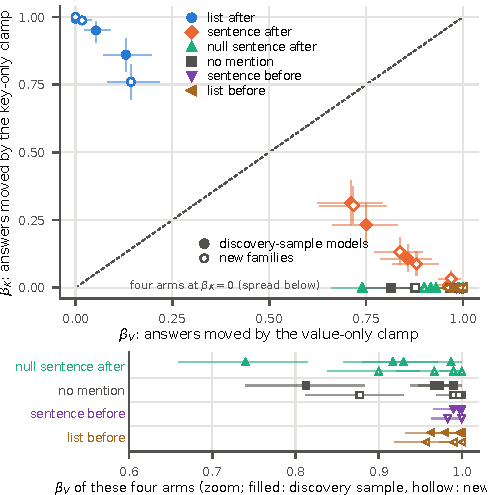
\includegraphics[width=0.8\textwidth]{figures/fig_crossover.pdf}
\caption{\textbf{Generated answers follow the channel the later mentions open} (fresh stories, eight models; the data of \cref{fig:schematic}c as a scatter). Each point is one model and arm: $\beta_K$, the share of generated answers that move to the clamped value under the key-only clamp, against $\beta_V$, the same under the value-only clamp, both net of moves to the clamped value under the clamp to the other of S and X; 95\,\% cluster intervals. The strip below spreads out the four arms whose $\beta_K$ is zero in every model (no mention, list before, sentence before, null sentence).}
\label{fig:crossover-full}
\end{figure}

\paragraph{The lines (J-B5, J-B5b).} With the list after the story, the key-only clamp moves \JbRangeBetaKAfterPfourMin{}--\JbRangeBetaKAfterPfourMax{} of generated answers to the clamped value in the discovery-sample models and \JbRangeBetaKAfterNfourMin{}--\JbRangeBetaKAfterNfourMax{} in the new families; without a mention, with the list before or with the sentence before, it moves none (\JbRangeBetaKNoneEightMax{}, \JbRangeBetaKBeforeEightMax{} and \JbRangeBetaKPreEightMax{} at most), and the value-only clamp moves \JbRangeBetaVNoneEightMin{}--\JbRangeBetaVNoneEightMax{} of answers without a mention (J-B5-P4f and J-B5-N4, held in \JbFivePfMet{} of \JbFivePfEval{} and \JbFiveNfMet{} of \JbFiveNfEval{}). The sentence read changes generated answers in seven of the eight models: the key-only clamp's flip rate is \JbFivebFlipPostMetMin{}--\JbFivebFlipPostMetMax{} after the sentence and \JbRangeFlipPreEightMax{} before it in those seven (J-B5b-N4, risky, held in \JbFivebNfMet{} of \JbFivebNfEval{}); at OLMo-2-7B the flip rate is \JbFivebFlipPostOlmoSeven{} after the sentence and \JbFivebFlipPreOlmoSeven{} before it, with a lower bound of \JbFivebLbOlmoSeven{} for the difference, so the discovery-sample line J-B5b-P4f was not met (risky; \JbFivebPfMet{} of \JbFivebPfEval{}). The record's reading (exploratory, recomputed): 3 of 150 items flip, in 3 of 55 cells, and 11.9\,\% of the resamples are exactly zero, so the failure does not depend on the seed; the key clamp under \fmtPost{} closes about 29\,\% of a 10-nat base--source margin at OLMo-2-7B, and the generations agree with the emitted-form argmax: the read is present in log-probabilities but too small to change OLMo-2's answers. The pre-written texts had no wording for this split; the wording used is a disclosed decision (\cref{app:decisions}). % verbatim: outcome J part B

\paragraph{The crossover (reported).} Over the eight models, $\beta_K$ under \fmtListA{} is \JbRangeBetaKAfterEightMin{}--\JbRangeBetaKAfterEightMax{} against $\beta_V$ = \JbRangeBetaVAfterEightMin{}--\JbRangeBetaVAfterEightMax{}; without a mention $\beta_V$ is \JbRangeBetaVNoneEightMin{}--\JbRangeBetaVNoneEightMax{} against $\beta_K$ = \JbRangeBetaKNoneEightMax{}; under \fmtPost{} $\beta_K$ is \JbRangeBetaKPostEightMin{}--\JbRangeBetaKPostEightMax{} and $\beta_V$ \JbRangeBetaVPostEightMin{}--\JbRangeBetaVPostEightMax{}; under \fmtNull{} $\beta_K$ is \JbRangeBetaKPostNullEightMax{} in every model and $\beta_V$ \JbRangeBetaVPostNullEightMin{}--\JbRangeBetaVPostNullEightMax{}. A single-channel clamp creates a cache state that no prompt produces; the generated answers show that the channel the later mentions open is the one that changes what the model says.

\subsection{Natural passages}\label{app:natural}

\paragraph{Design and gates.} Four models (Llama-3.1-8B and Gemma-2-9B, two families never examined before, and Qwen2.5-7B and Mistral-7B) answered the 185 counterfactual passages in six formats (\cref{app:prompts-natural}). Each line is decided on the items competent in its formats (the clean run answers B, the clamp to S answers S and the clamp to X answers X) and must hold in every evaluable model, with at least three evaluable models including a new family. Intervals are 95\,\% two-stage bootstrap intervals over articles and the items within them. Three gates decide evaluability (\cref{app:impl-j}). The BF16 floor failed in one cell, Llama-3.1-8B's options-after cell, by one item (generation agreement \JaGoneAgreeOptaLlamaEight{} against 0.97); every line that uses that cell is not evaluable in Llama. The competence floor of 80 items failed in five cells: Llama-3.1-8B with the related-articles sentence after and before the passage, and Mistral-7B in free form and with the sentence after and before. Mistral's free-form answers are mostly sentences (``The passage states that \ldots''), which the answer rule does not read as the entity, while its clamped answers never name B (exploratory, recomputed): a failure of answer form, not of compliance with the counterfactual. The emitted-form gate held in every cell (median probability of the decision token \JaGthreePMin{}--\JaGthreePMax{}; the first generated token was the decision token in at least \JaGthreeGoneMin{} of competent items). \Cref{tab:natural8} gives every model and format. % verbatim: outcome J part A

\begin{table}[!ht]
\centering
\caption{\textbf{Natural passages: identity by format.} Counterfactual SQuAD passages, 185 items per model; $n_{\mathrm{comp}}$: items competent in the format; $s_{\mathrm{ID}}$, $\mathrm{ID}_K$ and $\mathrm{ID}_V$ on those items, with 95\,\% two-stage article-cluster intervals. Gate: the preregistered gate that fails in the cell (J-A-G1: BF16 floor; J-A-G2: fewer than 80 competent items); such a cell enters no line. $^\dagger$Computed from the raw results with the scorer's functions, not printed by the scorer (exploratory).}
\label{tab:natural8}
\small
\setlength{\tabcolsep}{4pt}
\begin{tabular}{@{}llrcccl@{}}
\toprule
Model & Format & $n_{\mathrm{comp}}$ & $s_{\mathrm{ID}}$ & $\mathrm{ID}_K$ (nats) & $\mathrm{ID}_V$ (nats) & Gate \\
\midrule
Llama-3.1-8B & options after & 148 & \begin{tabular}[t]{@{}c@{}}0.524\\[-1pt]{\scriptsize[0.473, 0.568]}\end{tabular} & \begin{tabular}[t]{@{}c@{}}6.859\\[-1pt]{\scriptsize[5.903, 7.829]}\end{tabular} & \begin{tabular}[t]{@{}c@{}}6.237\\[-1pt]{\scriptsize[5.702, 6.805]}\end{tabular} & J-A-G1 \\
 & letters after & 156 & \begin{tabular}[t]{@{}c@{}}0.739\\[-1pt]{\scriptsize[0.675, 0.794]}\end{tabular} & \begin{tabular}[t]{@{}c@{}}6.726\\[-1pt]{\scriptsize[5.873, 7.572]}\end{tabular} & \begin{tabular}[t]{@{}c@{}}2.371\\[-1pt]{\scriptsize[1.805, 3.080]}\end{tabular} & -- \\
 & sentence after$^\dagger$ & 70 & \begin{tabular}[t]{@{}c@{}}0.075\\[-1pt]{\scriptsize[0.044, 0.106]}\end{tabular} & \begin{tabular}[t]{@{}c@{}}0.916\\[-1pt]{\scriptsize[0.514, 1.339]}\end{tabular} & \begin{tabular}[t]{@{}c@{}}11.260\\[-1pt]{\scriptsize[10.555, 11.969]}\end{tabular} & J-A-G2 \\
 & free form & 86 & \begin{tabular}[t]{@{}c@{}}0.045\\[-1pt]{\scriptsize[0.026, 0.063]}\end{tabular} & \begin{tabular}[t]{@{}c@{}}0.552\\[-1pt]{\scriptsize[0.315, 0.794]}\end{tabular} & \begin{tabular}[t]{@{}c@{}}11.786\\[-1pt]{\scriptsize[11.122, 12.434]}\end{tabular} & -- \\
 & options before$^\dagger$ & 164 & \begin{tabular}[t]{@{}c@{}}$-$0.023\\[-1pt]{\scriptsize[$-$0.035, $-$0.011]}\end{tabular} & \begin{tabular}[t]{@{}c@{}}$-$0.252\\[-1pt]{\scriptsize[$-$0.383, $-$0.121]}\end{tabular} & \begin{tabular}[t]{@{}c@{}}11.176\\[-1pt]{\scriptsize[10.440, 11.972]}\end{tabular} & -- \\
 & sentence before$^\dagger$ & 69 & \begin{tabular}[t]{@{}c@{}}$-$0.021\\[-1pt]{\scriptsize[$-$0.042, $-$0.002]}\end{tabular} & \begin{tabular}[t]{@{}c@{}}$-$0.227\\[-1pt]{\scriptsize[$-$0.429, $-$0.020]}\end{tabular} & \begin{tabular}[t]{@{}c@{}}10.784\\[-1pt]{\scriptsize[10.084, 11.531]}\end{tabular} & J-A-G2 \\
\midrule
Gemma-2-9B & options after & 158 & \begin{tabular}[t]{@{}c@{}}0.627\\[-1pt]{\scriptsize[0.599, 0.653]}\end{tabular} & \begin{tabular}[t]{@{}c@{}}9.868\\[-1pt]{\scriptsize[9.073, 10.596]}\end{tabular} & \begin{tabular}[t]{@{}c@{}}5.869\\[-1pt]{\scriptsize[5.379, 6.389]}\end{tabular} & -- \\
 & letters after & 158 & \begin{tabular}[t]{@{}c@{}}0.963\\[-1pt]{\scriptsize[0.927, 0.987]}\end{tabular} & \begin{tabular}[t]{@{}c@{}}9.676\\[-1pt]{\scriptsize[9.121, 10.128]}\end{tabular} & \begin{tabular}[t]{@{}c@{}}0.375\\[-1pt]{\scriptsize[0.132, 0.750]}\end{tabular} & -- \\
 & sentence after$^\dagger$ & 107 & \begin{tabular}[t]{@{}c@{}}0.067\\[-1pt]{\scriptsize[0.043, 0.092]}\end{tabular} & \begin{tabular}[t]{@{}c@{}}1.047\\[-1pt]{\scriptsize[0.653, 1.496]}\end{tabular} & \begin{tabular}[t]{@{}c@{}}14.685\\[-1pt]{\scriptsize[14.010, 15.349]}\end{tabular} & -- \\
 & free form & 109 & \begin{tabular}[t]{@{}c@{}}$-$0.003\\[-1pt]{\scriptsize[$-$0.010, 0.002]}\end{tabular} & \begin{tabular}[t]{@{}c@{}}$-$0.057\\[-1pt]{\scriptsize[$-$0.164, 0.037]}\end{tabular} & \begin{tabular}[t]{@{}c@{}}16.900\\[-1pt]{\scriptsize[16.204, 17.582]}\end{tabular} & -- \\
 & options before$^\dagger$ & 167 & \begin{tabular}[t]{@{}c@{}}$-$0.017\\[-1pt]{\scriptsize[$-$0.024, $-$0.011]}\end{tabular} & \begin{tabular}[t]{@{}c@{}}$-$0.183\\[-1pt]{\scriptsize[$-$0.262, $-$0.117]}\end{tabular} & \begin{tabular}[t]{@{}c@{}}11.234\\[-1pt]{\scriptsize[10.786, 11.692]}\end{tabular} & -- \\
 & sentence before$^\dagger$ & 117 & \begin{tabular}[t]{@{}c@{}}$-$0.018\\[-1pt]{\scriptsize[$-$0.024, $-$0.012]}\end{tabular} & \begin{tabular}[t]{@{}c@{}}$-$0.247\\[-1pt]{\scriptsize[$-$0.332, $-$0.164]}\end{tabular} & \begin{tabular}[t]{@{}c@{}}14.176\\[-1pt]{\scriptsize[13.500, 14.855]}\end{tabular} & -- \\
\midrule
Qwen2.5-7B & options after & 162 & \begin{tabular}[t]{@{}c@{}}0.677\\[-1pt]{\scriptsize[0.639, 0.715]}\end{tabular} & \begin{tabular}[t]{@{}c@{}}15.491\\[-1pt]{\scriptsize[13.983, 16.966]}\end{tabular} & \begin{tabular}[t]{@{}c@{}}7.385\\[-1pt]{\scriptsize[6.287, 8.550]}\end{tabular} & -- \\
 & letters after & 163 & \begin{tabular}[t]{@{}c@{}}0.935\\[-1pt]{\scriptsize[0.885, 0.972]}\end{tabular} & \begin{tabular}[t]{@{}c@{}}19.782\\[-1pt]{\scriptsize[18.416, 20.972]}\end{tabular} & \begin{tabular}[t]{@{}c@{}}1.366\\[-1pt]{\scriptsize[0.591, 2.438]}\end{tabular} & -- \\
 & sentence after$^\dagger$ & 106 & \begin{tabular}[t]{@{}c@{}}0.061\\[-1pt]{\scriptsize[0.027, 0.096]}\end{tabular} & \begin{tabular}[t]{@{}c@{}}1.335\\[-1pt]{\scriptsize[0.564, 2.144]}\end{tabular} & \begin{tabular}[t]{@{}c@{}}20.573\\[-1pt]{\scriptsize[19.205, 21.983]}\end{tabular} & -- \\
 & free form & 104 & \begin{tabular}[t]{@{}c@{}}0.014\\[-1pt]{\scriptsize[0.004, 0.025]}\end{tabular} & \begin{tabular}[t]{@{}c@{}}0.311\\[-1pt]{\scriptsize[0.081, 0.548]}\end{tabular} & \begin{tabular}[t]{@{}c@{}}21.430\\[-1pt]{\scriptsize[20.006, 22.911]}\end{tabular} & -- \\
 & options before$^\dagger$ & 166 & \begin{tabular}[t]{@{}c@{}}$-$0.053\\[-1pt]{\scriptsize[$-$0.067, $-$0.041]}\end{tabular} & \begin{tabular}[t]{@{}c@{}}$-$0.878\\[-1pt]{\scriptsize[$-$1.087, $-$0.671]}\end{tabular} & \begin{tabular}[t]{@{}c@{}}17.310\\[-1pt]{\scriptsize[16.163, 18.440]}\end{tabular} & -- \\
 & sentence before$^\dagger$ & 99 & \begin{tabular}[t]{@{}c@{}}$-$0.036\\[-1pt]{\scriptsize[$-$0.051, $-$0.022]}\end{tabular} & \begin{tabular}[t]{@{}c@{}}$-$0.725\\[-1pt]{\scriptsize[$-$0.993, $-$0.454]}\end{tabular} & \begin{tabular}[t]{@{}c@{}}20.770\\[-1pt]{\scriptsize[19.338, 22.218]}\end{tabular} & -- \\
\midrule
Mistral-7B & options after & 157 & \begin{tabular}[t]{@{}c@{}}0.550\\[-1pt]{\scriptsize[0.503, 0.593]}\end{tabular} & \begin{tabular}[t]{@{}c@{}}9.817\\[-1pt]{\scriptsize[8.568, 11.071]}\end{tabular} & \begin{tabular}[t]{@{}c@{}}8.029\\[-1pt]{\scriptsize[7.187, 8.907]}\end{tabular} & -- \\
 & letters after & 155 & \begin{tabular}[t]{@{}c@{}}0.786\\[-1pt]{\scriptsize[0.701, 0.864]}\end{tabular} & \begin{tabular}[t]{@{}c@{}}7.424\\[-1pt]{\scriptsize[6.211, 8.638]}\end{tabular} & \begin{tabular}[t]{@{}c@{}}2.016\\[-1pt]{\scriptsize[1.219, 2.987]}\end{tabular} & -- \\
 & sentence after$^\dagger$ & 43 & \begin{tabular}[t]{@{}c@{}}0.092\\[-1pt]{\scriptsize[0.009, 0.168]}\end{tabular} & \begin{tabular}[t]{@{}c@{}}1.545\\[-1pt]{\scriptsize[0.139, 3.045]}\end{tabular} & \begin{tabular}[t]{@{}c@{}}15.330\\[-1pt]{\scriptsize[14.205, 16.444]}\end{tabular} & J-A-G2 \\
 & free form & 43 & \begin{tabular}[t]{@{}c@{}}0.001\\[-1pt]{\scriptsize[$-$0.011, 0.015]}\end{tabular} & \begin{tabular}[t]{@{}c@{}}0.019\\[-1pt]{\scriptsize[$-$0.184, 0.257]}\end{tabular} & \begin{tabular}[t]{@{}c@{}}16.426\\[-1pt]{\scriptsize[15.215, 17.516]}\end{tabular} & J-A-G2 \\
 & options before$^\dagger$ & 150 & \begin{tabular}[t]{@{}c@{}}$-$0.026\\[-1pt]{\scriptsize[$-$0.037, $-$0.016]}\end{tabular} & \begin{tabular}[t]{@{}c@{}}$-$0.387\\[-1pt]{\scriptsize[$-$0.540, $-$0.240]}\end{tabular} & \begin{tabular}[t]{@{}c@{}}15.195\\[-1pt]{\scriptsize[14.444, 15.971]}\end{tabular} & -- \\
 & sentence before$^\dagger$ & 44 & \begin{tabular}[t]{@{}c@{}}$-$0.018\\[-1pt]{\scriptsize[$-$0.040, 0.000]}\end{tabular} & \begin{tabular}[t]{@{}c@{}}$-$0.278\\[-1pt]{\scriptsize[$-$0.586, 0.004]}\end{tabular} & \begin{tabular}[t]{@{}c@{}}15.313\\[-1pt]{\scriptsize[14.206, 16.307]}\end{tabular} & J-A-G2 \\
\bottomrule
\end{tabular}

\end{table}

\paragraph{Identity (J-A1--J-A5).} With options after the passage the key carries most of the answer entity's identity in the three evaluable models (J-A1, extrapolation, held: $s_{\mathrm{ID}}$ \JaSidOptaGemmaNine{}, \JaSidOptaQwenSeven{} and \JaSidOptaMistralSeven{} at Gemma-2-9B, Qwen2.5-7B and Mistral-7B, lower bounds above the preregistered 0.35; Llama-3.1-8B's cell, \JaSidOptaLlamaEight{}, not evaluable), also for answers of three or more tokens (J-A1b, risky, held: \JaOnebSidGemmaNine{} [\JaOnebSidGemmaNineLo{}, \JaOnebSidGemmaNineHi{}], \JaOnebSidQwenSeven{} [\JaOnebSidQwenSevenLo{}, \JaOnebSidQwenSevenHi{}] and \JaOnebSidMistralSeven{} [\JaOnebSidMistralSevenLo{}, \JaOnebSidMistralSevenHi{}]), and with lettered options in all four (J-A1c, held: $s_{\mathrm{ID}}$ \JaSidLetaLlamaEight{}--\JaSidLetaGemmaNine{}). In free form the value carries it (J-A2, held: $s_{\mathrm{ID}}$ \JaSidNomLlamaEight{}, \JaSidNomGemmaNine{} and \JaSidNomQwenSeven{} at Llama, Gemma and Qwen; Mistral not evaluable). The derived contrast J-A3 (options after minus free form at least 0.4; not counted) holds in both models where it is evaluable (\JaThreeDiffGemmaNine{} and \JaThreeDiffQwenSeven{}) and is not evaluable, because Llama's options-after cell and Mistral's free-form cell fail their gates. Options before the passage give a small negative key read in every model (J-A4, replication, held: $\mathrm{ID}_K$ \JaFourIDKOptbMin{} to \JaFourIDKOptbMax{} nats, ratios to the options-after read \JaFourRatioMin{} to \JaFourRatioMax{}); the line's criteria are one-sided. A related-articles sentence after the passage opens only a small key read: its gain in $s_{\mathrm{ID}}$ over free form is \JaFiveDiffGemmaNine{} at Gemma and \JaFiveDiffQwenSeven{} at Qwen, below the preregistered 0.10 (J-A5, risky, not held; Llama and Mistral not evaluable), although its key read is positive (\cref{tab:natural8}). Its contrast with the same sentence before the passage, J-A5B, holds in both evaluable models ($\mathrm{ID}_K$ difference \JaFiveBDiffGemmaNine{} and \JaFiveBDiffQwenSeven{} nats) and is not evaluable (two of the three required models).

\begin{table}[!ht]
\centering
\footnotesize
\caption{\textbf{Cue conflict and the copy fallback on passages.} The cache gets two sources: the key from one counterfactual entity and the value from another (S and X, both directions). Key / value: the share of generated answers naming the key's or the value's entity; ``other'': answers naming no candidate; dec.: the value-source rate at the decision token alone. Flag only: the key from S and the value from a third entity Z, share answering S; copy fallback: the key from Z and the value from S, share answering S. Whole answers; competent items; cells of Llama's options-after and Mistral's free-form formats fail a gate (not evaluable).}
\label{tab:cue}
\setlength{\tabcolsep}{4pt}
\begin{tabular}{@{}lccccccccc@{}}
\toprule
 & \multicolumn{2}{c}{options after} & \multicolumn{2}{c}{lettered options} & \multicolumn{3}{c}{free form} & flag only & copy fallback \\
\cmidrule(lr){2-3}\cmidrule(lr){4-5}\cmidrule(lr){6-8}
Model & key & value & key & value & value & other & value (dec.) & (options after) & (options after) \\
\midrule
Llama-3.1-8B & \JaKeySrcOptaLlamaEight{} & \JaValSrcOptaLlamaEight{} & \JaKeySrcLetaLlamaEight{} & \JaValSrcLetaLlamaEight{} & \JaValSrcNomLlamaEight{} & \JaOtherNomLlamaEight{} & \JaValSrcDecNomLlamaEight{} & \JaSixdOptaLlamaEight{} & \JaSixeSLlamaEight{} \\
Gemma-2-9B & \JaKeySrcOptaGemmaNine{} & \JaValSrcOptaGemmaNine{} & \JaKeySrcLetaGemmaNine{} & \JaValSrcLetaGemmaNine{} & \JaValSrcNomGemmaNine{} & \JaOtherNomGemmaNine{} & \JaValSrcDecNomGemmaNine{} & \JaSixdOptaGemmaNine{} & \JaSixeSGemmaNine{} \\
Qwen2.5-7B & \JaKeySrcOptaQwenSeven{} & \JaValSrcOptaQwenSeven{} & \JaKeySrcLetaQwenSeven{} & \JaValSrcLetaQwenSeven{} & \JaValSrcNomQwenSeven{} & \JaOtherNomQwenSeven{} & \JaValSrcDecNomQwenSeven{} & \JaSixdOptaQwenSeven{} & \JaSixeSQwenSeven{} \\
Mistral-7B & \JaKeySrcOptaMistralSeven{} & \JaValSrcOptaMistralSeven{} & \JaKeySrcLetaMistralSeven{} & \JaValSrcLetaMistralSeven{} & \JaValSrcNomMistralSeven{} & \JaOtherNomMistralSeven{} & \JaValSrcDecNomMistralSeven{} & \JaSixdOptaMistralSeven{} & \JaSixeSMistralSeven{} \\
\bottomrule
\end{tabular}
\end{table}

\paragraph{Behaviour (J-A6a--e).} \Cref{tab:cue} gives the cue-conflict rates. With lettered options the generated answer follows the key's entity in all four models (J-A6b, risky, held), and when the key matches no option the value is copied (J-A6e, risky, held in the three evaluable models). With options answered by name the key wins at Gemma and Qwen but not at Mistral (key-source rate \JaKeySrcOptaMistralSeven{} against the preregistered 0.6; J-A6a, risky, not held). In free form the value-source rate misses 0.6 at Llama and Qwen (J-A6c, risky, not held; Mistral not evaluable): many of the answers that name no candidate are hybrids that start with the value source's first word and do not complete the entity (34\,\% of the ``other'' answers at Llama to 76\,\% at Gemma; recomputed), and at the decision token the value-source rate is \JaValSrcDecNomMin{}--\JaValSrcDecNomMax{} while the key-source rate is at most 0.005. Scored on the answer's first word, which is not the preregistered criterion, the value-source rates would be 0.674 / 0.950 / 0.740 / 0.547 (Llama / Gemma / Qwen / Mistral; Llama's lower bound 0.55, exploratory, recomputed) and J-A6c would be met; as preregistered (the whole answer) it is not. The key-only flag (J-A6d) moves answers to the key's entity with options after the passage and never in free form in every model, but the line is not evaluable (two evaluable models). Llama's options-after cue conflict, whose cell is not evaluable, favours the value (key \JaKeySrcOptaLlamaEight{}, value \JaValSrcOptaLlamaEight{}), driven by numbers, 67 of its 70 single-token items, and by person names whose tokens are split between the key and the value source (exploratory, recomputed). Because J-A6a and J-A6c both failed, the hybrids are reported as an observation, not under the pre-written clause for a failure of J-A6c alone (\cref{app:decisions}), and the channel attributions are not shown to decide behaviour on natural text. % verbatim: outcome J part A

\paragraph{Continuations (J-A8, not evaluable; J-A8d, not held).} The continuation of a multi-token answer is read through an interaction of the two channels in all four models: in free form, the key and value effects on the continuation tokens add up to far less than the joint effect ($I_{\mathrm{cont}}$ = \JaIcontMin{}--\JaIcontMax{}), while at the decision token they add up ($I_{\mathrm{dec}}$ = \JaIdecMin{} to \JaIdecMax{}), and with options listed the joint clamp hardly moves the continuation (\JaContRatioMin{}--\JaContRatioMax{} of its free-form effect). The key alone moves the continuation away from S ($d_K^{\mathrm{cont}}$ = \JaDcontKMin{} to \JaDcontKMax{} nats), the pattern the line predicted: the key addresses the next piece and the value supplies it. This pattern is seen in all four models, but its line (J-A8, extrapolation) is not evaluable (two evaluable models: Llama's options-after cell fails the BF16 gate and Mistral's free-form cell the competence gate); it is a channel-level replication of induction-head K-composition \citep{elhage2021framework,olsson2022context}, not a novelty claim. The hybrid rate under a key that matches no candidate (J-A8d, risky) rests on Gemma alone, the one model with enough items (\JaEightdNomGemmaNine{} [\JaEightdNomGemmaNineLo{}, \JaEightdNomGemmaNineHi{}], 6 of 57 items, against 0.2), many of whose B entities are famous names that the model completes from memory; not held. % verbatim: outcome J part A

\paragraph{Quantization of the cached values (J-A7, J-A7b; exploratory reading).} The passage part also tested whether quantizing the passage's cached values to 2 bits with KIVI \citep{liu2024kivi} hurts free-form answers more than multiple-choice ones, beyond the same quantization of the keys. Only Qwen2.5-7B had enough prior-free items (33): the difference in differences was \JaSevenDiDQwenSeven{} [\JaSevenDiDQwenSevenLo{}, \JaSevenDiDQwenSevenHi{}] (J-A7, risky, not held) and the value drop's difference between formats \JaSevenbDiffQwenSeven{} [\JaSevenbDiffQwenSevenLo{}, \JaSevenbDiffQwenSevenHi{}] (J-A7b, risky, not held). The test had low power (the drops come from four and one items) and points the other way: on all competent items 2-bit keys cost free-form answers more than 2-bit values do (\cref{tab:kivi}), and neither costs multiple-choice answers (accuracy at least \JaKiviMcqMin{}). The relative reconstruction errors are \JaKiviErrKMin{}--\JaKiviErrKMax{} for the keys (per channel) and \JaKiviErrVMin{}--\JaKiviErrVMax{} for the values (per token), without strength matching. We make no claim about quantization. % verbatim: 33 items, outcome J part A

\begin{table}[!ht]
\centering
\footnotesize
\caption{\textbf{KIVI 2-bit quantization of the passage's cache} (exploratory). Faithful accuracy (the generation names S on the S passage) on competent items with no quantization, with 2-bit keys and with 2-bit values (every passage token, every layer; keys per channel, values per token, groups of 32), and the relative reconstruction errors $\lVert x' - x \rVert / \lVert x \rVert$.}
\label{tab:kivi}
\setlength{\tabcolsep}{5pt}
\begin{tabular}{@{}llccccc@{}}
\toprule
Model & Format & none & keys 2-bit & values 2-bit & error (keys) & error (values) \\
\midrule
Llama-3.1-8B & free form & \JaKiviNoneNomLlamaEight{} & \JaKiviKtwoNomLlamaEight{} & \JaKiviVtwoNomLlamaEight{} & \JaKiviErrKNomLlamaEight{} & \JaKiviErrVNomLlamaEight{} \\
 & options after & \JaKiviNoneOptaLlamaEight{} & \JaKiviKtwoOptaLlamaEight{} & \JaKiviVtwoOptaLlamaEight{} & \JaKiviErrKOptaLlamaEight{} & \JaKiviErrVOptaLlamaEight{} \\
 & lettered options & \JaKiviNoneLetaLlamaEight{} & \JaKiviKtwoLetaLlamaEight{} & \JaKiviVtwoLetaLlamaEight{} & \JaKiviErrKLetaLlamaEight{} & \JaKiviErrVLetaLlamaEight{} \\
\addlinespace[2pt]
Gemma-2-9B & free form & \JaKiviNoneNomGemmaNine{} & \JaKiviKtwoNomGemmaNine{} & \JaKiviVtwoNomGemmaNine{} & \JaKiviErrKNomGemmaNine{} & \JaKiviErrVNomGemmaNine{} \\
 & options after & \JaKiviNoneOptaGemmaNine{} & \JaKiviKtwoOptaGemmaNine{} & \JaKiviVtwoOptaGemmaNine{} & \JaKiviErrKOptaGemmaNine{} & \JaKiviErrVOptaGemmaNine{} \\
 & lettered options & \JaKiviNoneLetaGemmaNine{} & \JaKiviKtwoLetaGemmaNine{} & \JaKiviVtwoLetaGemmaNine{} & \JaKiviErrKLetaGemmaNine{} & \JaKiviErrVLetaGemmaNine{} \\
\addlinespace[2pt]
Qwen2.5-7B & free form & \JaKiviNoneNomQwenSeven{} & \JaKiviKtwoNomQwenSeven{} & \JaKiviVtwoNomQwenSeven{} & \JaKiviErrKNomQwenSeven{} & \JaKiviErrVNomQwenSeven{} \\
 & options after & \JaKiviNoneOptaQwenSeven{} & \JaKiviKtwoOptaQwenSeven{} & \JaKiviVtwoOptaQwenSeven{} & \JaKiviErrKOptaQwenSeven{} & \JaKiviErrVOptaQwenSeven{} \\
 & lettered options & \JaKiviNoneLetaQwenSeven{} & \JaKiviKtwoLetaQwenSeven{} & \JaKiviVtwoLetaQwenSeven{} & \JaKiviErrKLetaQwenSeven{} & \JaKiviErrVLetaQwenSeven{} \\
\addlinespace[2pt]
Mistral-7B & free form & \JaKiviNoneNomMistralSeven{} & \JaKiviKtwoNomMistralSeven{} & \JaKiviVtwoNomMistralSeven{} & \JaKiviErrKNomMistralSeven{} & \JaKiviErrVNomMistralSeven{} \\
 & options after & \JaKiviNoneOptaMistralSeven{} & \JaKiviKtwoOptaMistralSeven{} & \JaKiviVtwoOptaMistralSeven{} & \JaKiviErrKOptaMistralSeven{} & \JaKiviErrVOptaMistralSeven{} \\
 & lettered options & \JaKiviNoneLetaMistralSeven{} & \JaKiviKtwoLetaMistralSeven{} & \JaKiviVtwoLetaMistralSeven{} & \JaKiviErrKLetaMistralSeven{} & \JaKiviErrVLetaMistralSeven{} \\
\bottomrule
\end{tabular}
\end{table}

\paragraph{Reader heads on passages (J-A-HA1--HA3b, not evaluable).} The head lines needed Qwen2.5-7B and Mistral-7B. At Qwen2.5-7B the heads' BF16 floor failed ($\lvert m(\text{none}) - m(\text{clean})\rvert$ = \JaHaGoneNoneCleanQwenSeven{} nats against \JaHaGoneBoundQwenSeven{}): plain eager passes in different batch shapes differ by 0.7--0.9 nats at Qwen (0.1 at Mistral), and Qwen's eager teacher-forced chain fails in most items whose continuation contains the digit ``0'' (exploratory, recomputed), so every head line is not evaluable. The option rows are the readers in both models ($d_G/d_{\mathrm{full}}$ = \JaHaGtwoRatioQwenSeven{} and \JaHaGtwoRatioMistralSeven{}). At Mistral-7B, whose gates passed (exploratory): the top \JaHaKstarMistralSeven{} heads ranked on the passages recover $R$ = \JaHaOneRMistralSeven{} of the option rows' read and blinding them removes \JaHaOneKOMistralSeven{}, against \JaHaOneRrandMistralSeven{} and \JaHaOneKOrandMistralSeven{} for random sets; the reader heads found on the templated stories recover \JaHaTwoRMistralSeven{} and remove \JaHaTwoKOMistralSeven{} (\JaHaTwoOverlapMistralSeven{} heads shared with the natural set); and mean-ablating the natural set at every row after the question lowers faithful multiple-choice accuracy on prior-free items by \JaHaThreeaDropMistralSeven{}. Ablating the heads with the largest direct effect on the answer in free form (a copy set) breaks both formats (faithful accuracy with options after \JaAblFaithNoneOptaQwenSeven{} $\to$ \JaAblFaithCstarOptaQwenSeven{} at Qwen and \JaAblFaithNoneOptaMistralSeven{} $\to$ \JaAblFaithCstarOptaMistralSeven{} at Mistral; in free form \JaAblFaithNoneNomQwenSeven{} $\to$ \JaAblFaithCstarNomQwenSeven{} and \JaAblFaithNoneNomMistralSeven{} $\to$ \JaAblFaithCstarNomMistralSeven{}), and ablating the natural readers also lowers free-form accuracy (to \JaAblFaithNstarNomQwenSeven{} and \JaAblFaithNstarNomMistralSeven{}; exploratory): the readers found at the option rows are needed for free-form answers as well. Because ablating the readers and cutting their attention disagree on whether the copy route takes over in the discovery sample (\cref{app:heads}), these passage tests would have bridged the two; they are not evaluable. % verbatim: outcome J part A

\paragraph{Sensitivity: Llama's options-after cell (disclosed).} Had the BF16 gate passed in that cell (180 of 185 items instead of 179), J-A3 would be met (three evaluable models including a new family) and J-A6d not met (Llama's flag-only rate \JaSixdOptaLlamaEight{} against 0.6); J-A1, J-A4, J-A6a and J-A6e would not change, and the risky tally of this part would read 3 of 10 (expected 4.65). % verbatim: outcome J part A

\paragraph{Holm sensitivity.} Over the 43 interval components of this part's risky lines, Holm's step-down changes one decision, J-A5's component at Qwen2.5-7B ($p$ = \JaHolmP{} against a threshold of \JaHolmThr{}), and no verdict. J-A6b's Mistral component passes Holm by a relative margin of 0.2\,\% ($p$ 0.002772 against 0.002778), within the Monte Carlo error of the bootstrap standard error, so J-A6b should not be described as robust to Holm. % verbatim: outcome J part A

\paragraph{Reported and exploratory.} Without the passage, the question and options alone favour the original answer: the closed-book argmax is $e_B$ in \JaPriorOptMin{}--\JaPriorOptMax{} of items (persons \JaPriorOptPersonMin{}--\JaPriorOptPersonMax{}, numbers \JaPriorOptNumberMin{}--\JaPriorOptNumberMax{}); the identity measures are contrasts between S and X, from which this prior cancels to first order. On all 185 valid items (not only competent ones) the pattern is the same: $s_{\mathrm{ID}}$ with the sentence after the passage is \JaSidAllMenaMin{}--\JaSidAllMenaMax{}, and with options or the sentence before it \JaSidAllBeforeMin{} to \JaSidAllBeforeMax{}; the option mass at the decision token is \JaMassAllListMin{}--\JaMassAllListMax{} with the options listed and \JaMassAllNoListMin{}--\JaMassAllNoListMax{} without. In the LEAK stratum (a surname re-mentioned in the passage after the full name; 65 items) $s_{\mathrm{ID}}$ is \JaLeakSidNomMin{}--\JaLeakSidNomMax{} in free form and \JaLeakSidOptaMin{}--\JaLeakSidOptaMax{} with options after. This says nothing about whether a natural in-passage re-mention opens a key read: the S, X and Z passages differ from B only inside the answer span, so the re-mention still names the original entity, and its match to a foreign key is lost alike under S and X and cancels in the S-versus-X contrast of \cref{eq:idk}. A test needs the counterfactual written at every mention (\cref{sec:limitations}, (i)). On years (80 items), at the first digit that differs, the free-form read is value-only ($d_K$ \JaEfourDKNomMin{} to \JaEfourDKNomMax{} nats against $d_V$ \JaEfourDVNomMin{}--\JaEfourDVNomMax{}), and with options listed the key reads ($d_K$ \JaEfourDKOptaMin{}--\JaEfourDKOptaMax{}), against the written expectation, which was value-only for both formats. Scored on the full answer string from the decision token on, $s_{\mathrm{ID}}$ in free form is negative (\JaEsixSidNomMin{} to \JaEsixSidNomMax{}), the continuation pattern above. With the clamp started at 30\,\% of the depth the free-form value copy keeps \JaEoneOnNomMin{}--\JaEoneOnNomMax{} of its full effect, while the options-after key read keeps \JaEoneOnOptaMin{}--\JaEoneOnOptaMax{}; the first span piece carries \JaEoneFirstNomMin{}--\JaEoneFirstNomMax{} of the value copy, while the later pieces carry \JaEoneRestOptaMin{}--\JaEoneRestOptaMax{} of the key read (the first \JaEoneFirstOptaMin{}--\JaEoneFirstOptaMax{}). All of these are exploratory. % verbatim: 65 and 80 items, entry J part A
